\documentclass{UCreport} 



\usepackage[authoryear,comma,round]{natbib}
\usepackage{hyperref,graphicx}
\usepackage{datatool,booktabs,pgfplotstable}
\usepackage[separate-uncertainty=true,multi-part-units=single]{siunitx}

\usepackage{caption}
\usepackage[list=true,listformat=simple]{subcaption}
\makeatletter
\g@addto@macro\p@subfigure{.}
\makeatother


\usepackage{chngcntr}

\usepackage[para]{footmisc}

\usepackage[super]{nth}

\usepackage{amsmath,amssymb}

\DeclareSIUnit{\arcsec}{''}
\DeclareSIUnit{\au}{\mathrm{AU}}
\DeclareSIUnit{\mag}{\mathrm{mag}}
\DeclareSIUnit{\px}{\mathrm{px}}

\usepackage[utf8]{inputenc}
\usepackage[T1]{fontenc}
\usepackage{newunicodechar}

\DeclareRobustCommand{\okina}{%
  \raisebox{\dimexpr\fontcharht\font`A-\height}{%
    \scalebox{0.8}{`}%
  }%
}
\newunicodechar{ʻ}{\okina}
\newcommand{\omuamua}{\okina Oumuamua } %space needed to get next word spaced 
\newcommand{\omuamuans}{\okina Oumuamua} %no space after

\pgfplotsset{compat=1.18}
\renewcommand*\dtldisplaystarttab{\toprule}
\renewcommand*\dtldisplayendtab{\tabularnewline\bottomrule}
\renewcommand*\dtldisplayafterhead{\midrule}
\pgfplotstableset{
    every head row/.style={before row=\toprule, after row=\midrule},
    every last row/.style={after row=\bottomrule}
}

\begin{document}



%----------- Report information ---------

\logo{logos/UC.png}
\school{\textbf{School of Physical and Chemical Sciences}}
\course{\textbf{ASTR480}}
\student{\textbf{Brayden Leicester}}
\supervisor{Dr Michele Bannister \\ and Dr Ryan Ridden-Harper}
\ttitle{Asteroids in TESS} %title of the file


%----------- Init -------------------

\buildmargins % display margins
\buildcover % create the front cover of the document



%------------ Declaration ----------------
\pagenumbering{roman}
\addcontentsline{toc}{section}{Declaration}
\declaration

I certify that content of this report was mostly my own work.
\\

My supervisors helped by proofreading the report and offering feedback. As well as providing useful insight into problems when I was stuck.\\

\autoref{Fig:FreqVsDiam} has been recreated after data from the Light Curve Database (LCDB) \citet{Warner2009}, as cited in text. That data has been supplemented with my own work in the corresponding \autoref{Fig:FreqDiamUpdate}.\\

\autoref{Eq:LCModel} was adapted from the \texttt{Astropy} documentation
\citep{Astropy2022} ( \url{https://docs.astropy.org/en/stable/api/astropy.timeseries.LombScargle.html#astropy.timeseries.LombScargle.model_parameters}) for how the model is fit to the data. \\

The TESS data was reduced for me by \texttt{TESSreduce} as part of the \texttt{TESSELLATE} pipeline, but the photometry is my own.
All the analysis of the photometry was also done by me. 

\vspace{2cm}
\begin{centering}
  \textbf{\student}\par
\end{centering}

\newpage

%------------ Abstract ----------------

\addcontentsline{toc}{section}{Abstract}
\abstract

% %*Background
The Transiting Exoplanet Survey Satellite (TESS) is a wealth of high-cadence photometric data. 
Asteroids move across the TESS field, and their intrinsic rotation varies their brightness periodically. 
Here, I present an analysis of the asteroids in TESS sector 29, as an addition to the \texttt{TESSELLATE} pipeline's analysis.

% %*Methods
After obtaining the positions of the asteroids in \qty{12}{\hour} intervals, they are interpolated to match the cadence of the TESS images (\qty{10}{\min}).
Aperture photometry of the asteroids is performed to construct a lightcurve.
The rotation periods and amplitudes are calculated by a Lomb-Scargle periodogram.
Quality checks are applied to properties of both the lightcurve and the periodogram of each object, to ensure accurate quantities are calculated. 
Comparing derived values for objects with known periods, it is found that \qty{70}{\percent} of the detected periods are reliable.

% %*Main Results
5664 asteroids are found in the sector, of which 374 passed all the quality checks.
\qty{80}{\percent} of these have no known period. 
The distribution of periods and amplitudes broadly agrees with other analyses of TESS data.
While some asteroids are calculated to have a large amplitude of variation, manual checking determined this to be an artefact of data contamination.
It is shown that more than half of the objects with a visual magnitude above \qty{16.36(0.73)}{\mag} have reliable periods detected.

% %*Conclusion
While only one sector is analysed here, the methods are shown to be robust and can now be run on any TESS sector. 

\newpage
%------------ Contents pages ----------------

\toc % creates the table of contents

\addcontentsline{toc}{section}{List of Figures}
\listoffigures
\newpage
\addcontentsline{toc}{section}{List of Tables}
\listoftables
\newpage

%------------ Report body ----------------
\pagenumbering{arabic}

\section{Introduction}\label{Sec:Intro}

%To get all asteroids in TESS. 
This project aims to find and characterise the light curves of all the asteroids seen by the Transiting Exoplanet Survey Satellite (TESS).
Combining knowledge of these asteroids positions with the high-cadence imaging of TESS should allow for the determination of rotation periods of these small bodies, and the amplitude of the variation in their lightcurves.


\subsection{Asteroids}\label{SubSec:Asteroid}

Asteroids are a key class of solar system objects. Much is known about them already, but there is always more to learn.
Three values characterise the orbits of asteroids, the proper elements of the object.
These are the length of the long axis of the orbit, the semi-major axis, $a$, how elliptical the orbit is, the eccentricity, $e$, and the angle to the ecliptic plane, the inclination, $i$.
Typical values for main belt asteroids are an $a$ of \qtyrange{2}{3.3}{\au}, an $e$ in \qtyrange{0}{0.35}{} and an $i$ around \qtyrange{0}{30}{\degree} \citep{DeMeo2015}.
Comets have undefined $a$ and larger $e$, with some long-period comets having $e\approx 1$, but the typical range is \qtyrange{0.2}{0.7}{} \citep{Lewis2012}.
Interstellar objects (ISOs) have $e>1$ as they are on unbound hyperbolic trajectories \citep{McGlynn1989}.


% The semi-major axis, $a$, is the largest distance from the sun that the asteroid achieves on its elliptical orbit.
% Main belt asteroids have a typical $a$ of \qtyrange{2}{3.3}{\au} \citep{DeMeo2015}.
% The bounds between the inner, middle and outer main belt at \qty{2.5}{\au} and \qty{2.82}{\au}, these separations are due to resonances with Jupiter (the 3:1 and 5:2 mean motion resonances mark the edges of middle main belt) and Saturn (the $\nu_6$ secular resonance cuts off the lowest $a$ edge of the inner belt) carving swathes where asteroids cannot be in stable orbits.

% The eccentricity, $e$, of this orbit is the next proper element. $e=0$ implies a perfectly circular orbit, $0<e<1$ are ellipses, $e=1$ give a parabolic orbit, and $e>1$ are unbound, hyperbolic orbits.
% Main belt asteroids have small $e$, in the range of  \citep{DeMeo2015}
% Comets have larger $e$, with some long period comets having $e\approx 1$, but the typical range is \qtyrange{0.2}{0.7}{} \citep{Lewis2012}.
% Interstellar objects (ISOs) have $e>1$ as they are on unbound hyperbolic trajectories.

% The inclination, $i$, of asteroids is also a key orbital element, it is the angle relative to the ecliptic plane.
% In principle asteroids can span the whole range of inclinations, though they rarely do.
% Main belt asteroids have typical inclinations of \qtyrange{0}{30}{\degree} \citep{DeMeo2015}, so the TESS cameras closer to the ecliptic plane are expected to have the most asteroids in their fields.

Asteroids can be grouped into families based on  the  clustering of the proper orbital elements and similarities in their colour or spectra \citep{Nesvorny2015}.
These families are named for their largest member.
Families are thought to all originate from the same body that was destroyed by a collision earlier in the solar system's history.

%TODO Rotation of asteroids
As an asteroid rotates, the amount of sunlight reflected changes with time.
This produces a lightcurve that is often sinusoidal in appearance.
These lightcurves are normally ``double-peaked'', with two maximums for one full rotation, due to symmetries in the object's shape. 
The shape of the asteroid has a large effect on the scale of variation in the lightcurve \citep{Durech2015}, the more elongated the object is, the larger the variation.
The rate of rotation is limited by the size of the asteroid \citep{Pravec2000}, as the body's internal strength is placed under too much strain if large
asteroids rotate with short periods.

Understanding the rotation properties of asteroids has long been of interest to astronomers \citep[e.g.][for early work into the limits of rotation period and the tumbling nature of some small bodies]{Weidenschilling1981,Harris1994}.
This is still at the forefront of research, with more lightcurves being published year-on-year \citep{Harris2015}.
For the smallest objects ingenious observation techniques are employed to measure rotation periods such as intentionally streaking the asteroid down a column of pixel on a detector, and making a lightcurve from the streak, as done by \citet{Bolin2023}.

Asteroids can have their rotation properties changed with time, collisions can do this, and so can light from the sun.
The YORP effect (named for the discoverers Yarkovsky, O'Keefe, Radzievskii, and Paddack) is the process of torquing asteroids of an asymmetric shape by both bombardment of photons and thermal (re-)emission \citep{Rubincam2000}.

The long cadence data on solar system bodies will only increase with more large survey telescopes coming online soon, such as the Legacy Survey of Space and Time \citep[LSST][]{LSST2019}.
The number of new asteroids that are well characterised will increase by more than 2 orders of magnitude on the Sloan Digital Sky Survey \citep[SDSS][]{York2000} which had $\sim 88000$ objects \citet{Parker2008}.
LSST needs a dedicated pipeline for asteroid classification, the Solar System Notification Alert Processing System \citep[SNAPS][]{Trilling2023} has been developed using Zwicky Transient Facility \citep[ZTF, ][]{Bellm2018} data and can scale up to handle the volume of data from LSST.
Work is being done to understand the biases of how  asymmetric shape high amplitude variations can lead to selection effects of such a large sample of asteroids \citet{Levine2023}.

Because of such a rich history of study, many asteroids have a known rotation period.
These are catalogued by \citet{Warner2009} in the Light Curve Database (LCDB).
In the October \nth{1}, 2023 release, the LCDB has nearly 9000 objects with periods determined to a quality code $U\geq 2-$, which is the minimum reliability recommended by \citeauthor{Warner2009} for statistical analysis.
This includes other TESS data from \citet{Pal2020} and \citet{Woods2021}.
A frequencies and diameter plot of these asteroids in \autoref{Fig:FreqVsDiam} shows the collection of all the asteroids in the LCDB with $U\geq 2-$.
The diameter presented in the LCDB here is calculated from the absolute magnitude, $H$, of the bodies, assuming an albedo.
\citeauthor{Warner2009} acknowledge that there are direct measurements of diameter for more asteroids in the present day, but continue to present the $H$-derived diameters for consistency.

The asteroid spin barrier \citep{Pravec2000} is seen in the red dashed lines in \autoref{Fig:FreqVsDiam}.
There are very few asteroids larger than $\qty{0.15}{\kilo\metre}$ rotating faster than $\sim \qty{10}{\per\day}$.
It is thought that the YORP effect, as well as collisions, spin up asteroids so fast that they pass above this barrier and then no longer have the internal strength necessary to hold themselves together.
This implies that all asteroids made to spin faster have torn themselves apart because they have no tensile strength, i.e. they are rubble piles instead of monoliths \citep{Harris1996}.
This idea of the cohesive strength of small bodies is still explored today \citep[e.g.][for V-type asteroids]{Oszkiewicz2020}.

Comparing the periods I calculate for asteroids already in the LCDB is an important sanity check of my methods, and ensures the periods calculated for asteroids for which no data exists are reliable.

\begin{figure}[h]
  \centering
  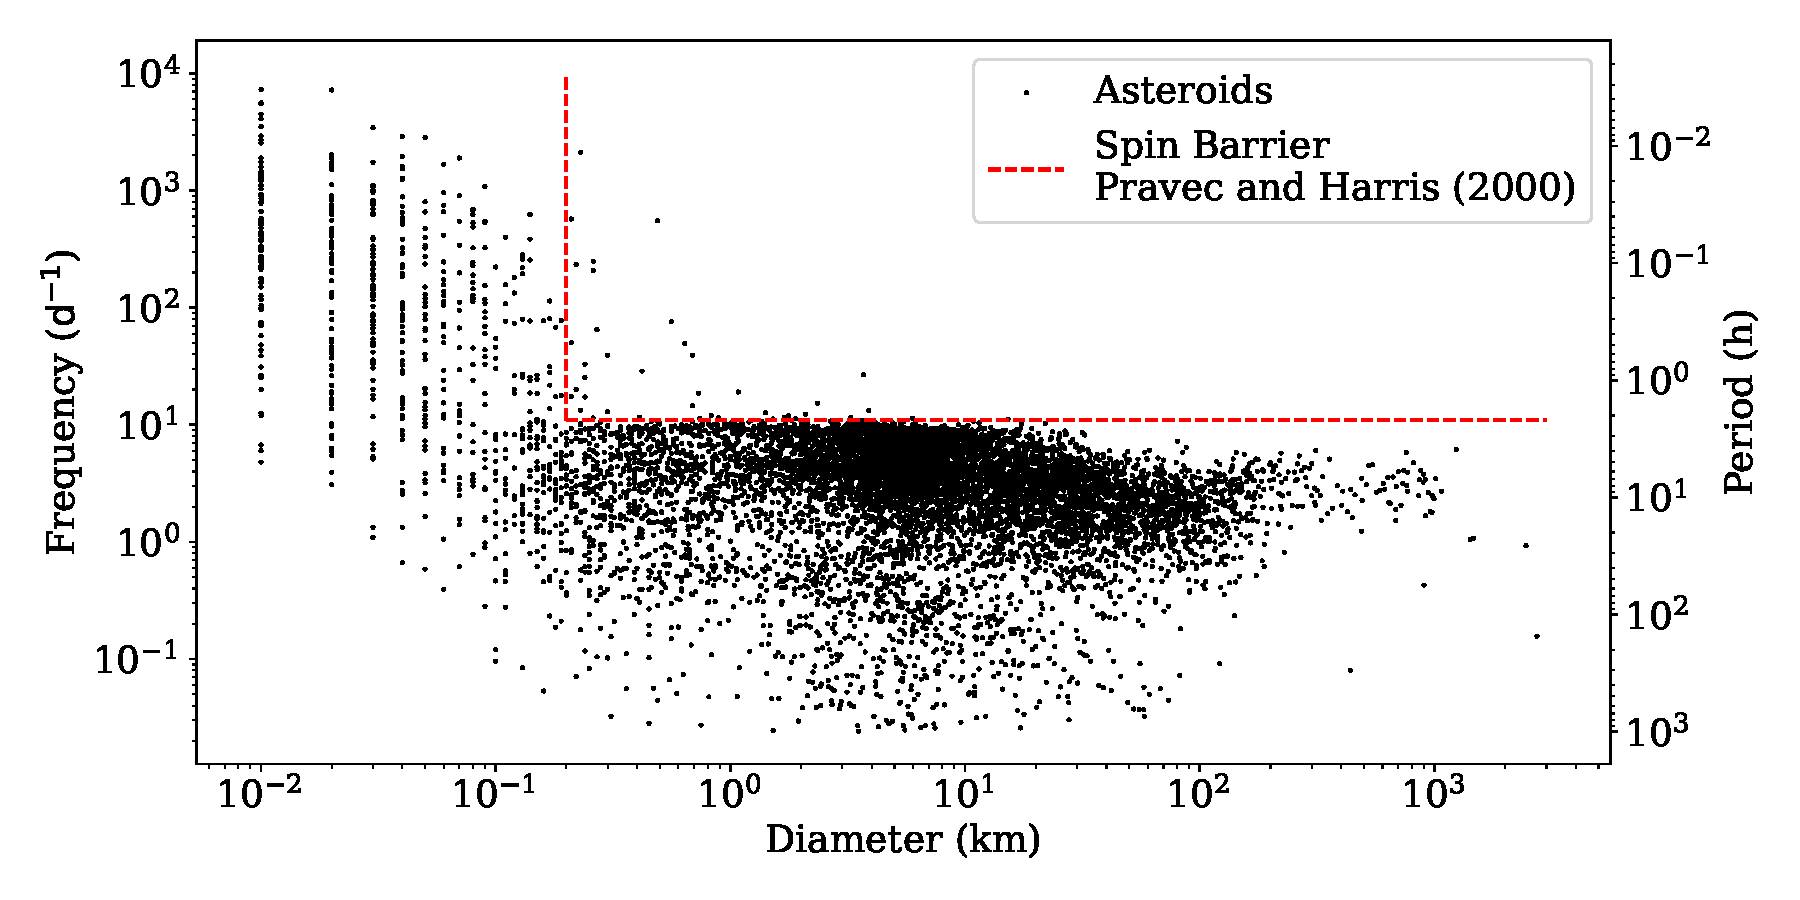
\includegraphics[width=0.7\textwidth]{./Figures/Diam-FreqPlot.pdf}
  \caption[Asteroid frequencies against diameter (LCDB)]{
    Rotation rate of asteroids by their size, recreated from the  October \nth{1}, 2023 LCDB after \citet{Warner2009}.
  }
  \label{Fig:FreqVsDiam}
\end{figure}

\subsubsection*{Interstellar Objects}
High amplitude variation has come to the forefront of questions about asteroid properties because of the first interstellar object, 1I/\omuamua \citep[see][for a review]{Bannister2019}.
\omuamua was determined to be spectroscopically red \citep{Fitzsimmons2017, Meech2017}, and having a photometric colour in the neutral end of the solar system range \citep{Bannister2017}.
1I was classed as an asteroid due to lack of a coma, and no noticeable activity.
This contrasts the second ISO, 2I/Borisov, which had many cometary characteristics \citep[see ][for a review]{Dorofeeva2023}.

\omuamua was measured to have a rotation period of \qty{8.67(0.34)}{\hour} \citep{Belton2018} and seemed to be tumbling \citep[e.g.][]{Drahus2018,Fraser2018}.
Combing the tumbling with an elongation ratio of up to \qty{6(1)}{}:1 \citep{McNeill2018}, 1I is said to have a cigar shape \citep{Belton2018}.
The peak to peak amplitude variation of this ISO was \qty{2.5}{\mag} \citep{Meech2017} over its double-peaked lightcurve, which is interesting as it is more variation than most asteroids more than most asteroids \citep[as seen in the LCDB of][]{Warner2009}.
With the full sky survey of bright asteroids, I aim to see how rare \omuamua is, by finding asteroids with large amplitude variations.


\subsection{TESS}\label{SubSec:TESS}

%Why TESS
TESS is a large area, high-cadence imaging, space telescope  \citep{Ricker2014}.
TESS is tasked with observing one piece of sky for \qty{27}{\day} at a time, which defines a sector.
The telescope delivers \qtyproduct{96 x 24}{\degree} full frame images (FFIs).
These FFIs are built from stacked \qty{2}{\second} exposures, leveraging the short readout times of the 16 charged-coupled devices (CCDs) spread over four cameras.
With the initial cadence for these full frame images set to \qty{30}{\minute}, the time resolution of TESS is unparalleled.
As the mission was extended after TESS had already mapped the entire sky, the length of the FFIs decreased to \qty{10}{\minute} and then later to \qty{200}{\second}.
This high time resolution and observation area does come at the cost of spatial resolution, as the pixels are each \qty{21}{\arcsec} square.

Of interest here is what such a high sampling rate can do for statistics on the asteroid population.
Rotation periods of bright asteroids can be easily determined from this vast dataset, due to the high sampling of the lightcurve.
The shortest FFIs will be able to accurately determine the rotation periods of all but the fastest rotating asteroids, most of which will be too dim to see in the TESS data.

The highest frequency (the shortest period) that can be found from time series data is the Nyquist limit, twice the minimum time between images \citep{VanderPlas2018}. 
Due to the short cadence, the Nyquist frequency of TESS is quite high, \qty{1}{\per\hour}.
This is well sampled enough to characterise most variable stars and determine the orbital periods of exoplanets to high precision.
The decrease in the FFI exposure time in later sectors comes with a complementary increase in the Nyquist frequency.

Previous work has been conducted to find and classify all the asteroids in TESS data.
\citet{Pal2018} propose that TESS will be a good instrument for solar system object study, a sentiment shared by \citet{Wong2019}.
\citeauthor{Pal2018} simulate some detections down to \nth{20} visual magnitude and find good photometry should only be expected to $V \lesssim 19$.
The first data release in \citet{Pal2020} catalogues nearly 10,000 asteroid lightcurves from the first year of TESS operation (cycle 1) with the \qty{30}{\min} cadence, and they report that they triple the number of asteroids with accurate rotation periods.
The Minor Planet Center (MPC) gets regular updates from TESS because of the work of \citet{Woods2021} and their \texttt{LINEAR-TESS} program, which creates tracklets of objects over a day, and then stitches these together to form a track of each asteroid through an FFI.

\citet{McNeill2023} also analyse TESS cycle 1, and detect almost 38,000 objects.
They determine reliable rotation periods for about 3,500 asteroids in this sample and show a lack of reliability for objects with periods less than \qty{3}{\hour}.
In the overlap from the data from \citet{Pal2020}, \citeauthor{McNeill2023} find good agreement between the two sets of periods and amplitudes.

There is ongoing analysis of subsets of the asteroid population in TESS.
\citet{Gowanlock2024} use TESS photometry as well as  observations by ZTF to get a longer baseline on mutually observed objects while combining ground and space-based observations.
There were a limited number of objects in both samples with known periods for comparison, with only 222 objects analysed. However, they demonstrate that the technique is effective.
Fainter and unknown solar system objects can be found by shift and stacking \citep{Holman2019, Payne2019,Rice2020} or taking a fast X-ray transform \citep{Nguyen2024} of the FFI data. 

This work aims to extend these other TESS studies to more sectors and examine the higher cadence FFIs, hence characterising more asteroids.
The goal is to get a volume complete set of asteroid lightcurves and periods, by analysis of the whole sky as seen by TESS using data from more than just the first year of TESS's operation.
This has not been achieved, as the analysis of only one sector is presented here, but the methods are scalable.

\section{Methods}\label{Sec:Meth}

Because of the survey properties, TESS provides a self-consistent way to measure the properties of asteroids over the full sky.
By using the higher cadence FFIs of later TESS sectors, the $P\leq\qty{3}{\hour}$ limit on the accurate periods \citep[as found by ][]{McNeill2023} can be lowered.
I also employ a different data reduction method, using reduced data from the \texttt{TESSreduce} package \citep{Ridden-Harper2021}.
This should increase the accuracy of the photometry due to the improved background subtraction process.

This work is part of a full sky transient survey using TESS, the TESS Extensive Lightcurve Logging and Analysis of Transient Events (\texttt{TESSELLATE}) pipeline \citep{TESSELLATE}.
To see what \texttt{TESSELLATE} detects and to help progress the pipeline, one can participate in the Cosmic Cataclysms Zooniverse project\footnote{\href{https://www.zooniverse.org/projects/cheerfuluser/cosmic-cataclysms}{https://www.zooniverse.org/projects/cheerfuluser/cosmic-cataclysms}}.

Asteroids can spike the brightness of a pixel for only a few frames while it is passing by.
When the pipeline is looking for transients such as flare stars and supernovae, asteroids can look very similar.
There is a brightness change in one pixel for a short time, as the object moves through the field.
Finding the asteroids will allow for these spikes to be filtered from the transient pipeline, while also gaining a better understanding of the asteroid population.
By filtering the asteroid detections out, while also self-consistently determining the rotation properties of a large sample of the population, more science can be done with one set of analyses.

The \texttt{TESSELLATE} pipeline has been running on the OzSTAR supercomputing facilities.
I built this asteroid detection and subsequent lightcurve and periodogram analysis program by testing one subsection of one CCD of one camera  of one TESS sector.
The code written can be accessed at my ASTR480 GitHub repo \footnote{\href{https://github.com/ble61/ASTR480}{https://github.com/ble61/ASTR480}}.
Because of the large number of asteroids there are too many lightcurves to look at, so the code has to run with no human decisions.
Once I was confident this worked as required, the same code was refactored slightly to work on OzSTAR and a large-scale analysis of a processed TESS sector was run.
I have been looking for completeness of detections of asteroids in \texttt{TESSELLATE}, as well as accuracy of periods and amplitude variation calculated.

Here, I present an analysis of TESS sector 29\footnote{\url{https://tess.mit.edu/observations/sector-29/}}, which was observed between \nth{26} August and \nth{22} September 2020.
Sector 29 was the third TESS sector employing \qty{10}{\min} FFIs and this cadence has been focused on less in the literature. 
It was chosen because it was the only sector of this cadence that had been processed by TESSELLATE with enough time for my analysis to be performed. However, what is presented in this section is scalable
on a per-sector basis to any sector that has been reduced. 


\subsection{Querying Databases for Asteroid Positions and Properties}\label{SubSec:Querry}

To check for asteroids in the TESS data, the positions of the asteroids with time are required.
For asteroids bright enough to be in TESS, their ephemeris is well known, so I needed to access their positions and then cross-match them with transients in the TESS data.

The sky body tracker, \texttt{SkyBoT} \citep{Berthier2006}, was queried to get the positions of asteroids.
A box in right ascension (RA) and declination (Dec) space was drawn on the sky, centred in the middle of each subsection made by \texttt{TESSELLATE} and a cone search was executed by \texttt{SkyBoT}.
The search was limited to only asteroids with an average visual magnitude $V\geq \qty{20}{\mag}$ because of the analysis of \citet{Pal2018}.
As TESS sectors are \qty{27}{\day} long, querying every \qty{12}{\hour} is computationally feasible and also allows for a good understanding of a body's motion.

Knowing where the asteroids were helped to find them in the archival TESS data, but knowing more about the individual asteroids is also useful for population statistics.
The \texttt{Astroquery} \citep{Ginsburg2019} package was used to query \texttt{JPL Horizons} was used to obtain the orbital elements of each asteroid, $a$, $e$, and $i$, as well as an absolute magnitude $H$.
The proper elements do not change with the asteroid's positions in its orbit, so only one query is needed per object. 

\subsection{Interpolation of the Positions to Match TESS Cadence}\label{SubSec:Interp}

\begin{figure}[t!]
  \centering
  \includegraphics[width =0.8 \textwidth]{./Figures/interpPos\_29\_1\_2\_2.pdf}
  \caption[Interpolated Positions of Asteroids on Sky]{
    The interpolated positions of asteroids in one subsection of a TESS sector.
    The colours of the lines are time sequenced, as shown in the colour bar.
    The alpha of the colours are scaled by the absolute magnitude $H$ of the asteroid.
    Both celestial coordinates (RA and Dec) and ecliptic longitude and latitude  axes are shown.
    The green $+$ is the centre of the subsection.}
  \label{Fig:interpPos}
\end{figure}


\begin{figure}[t]
  \centering
  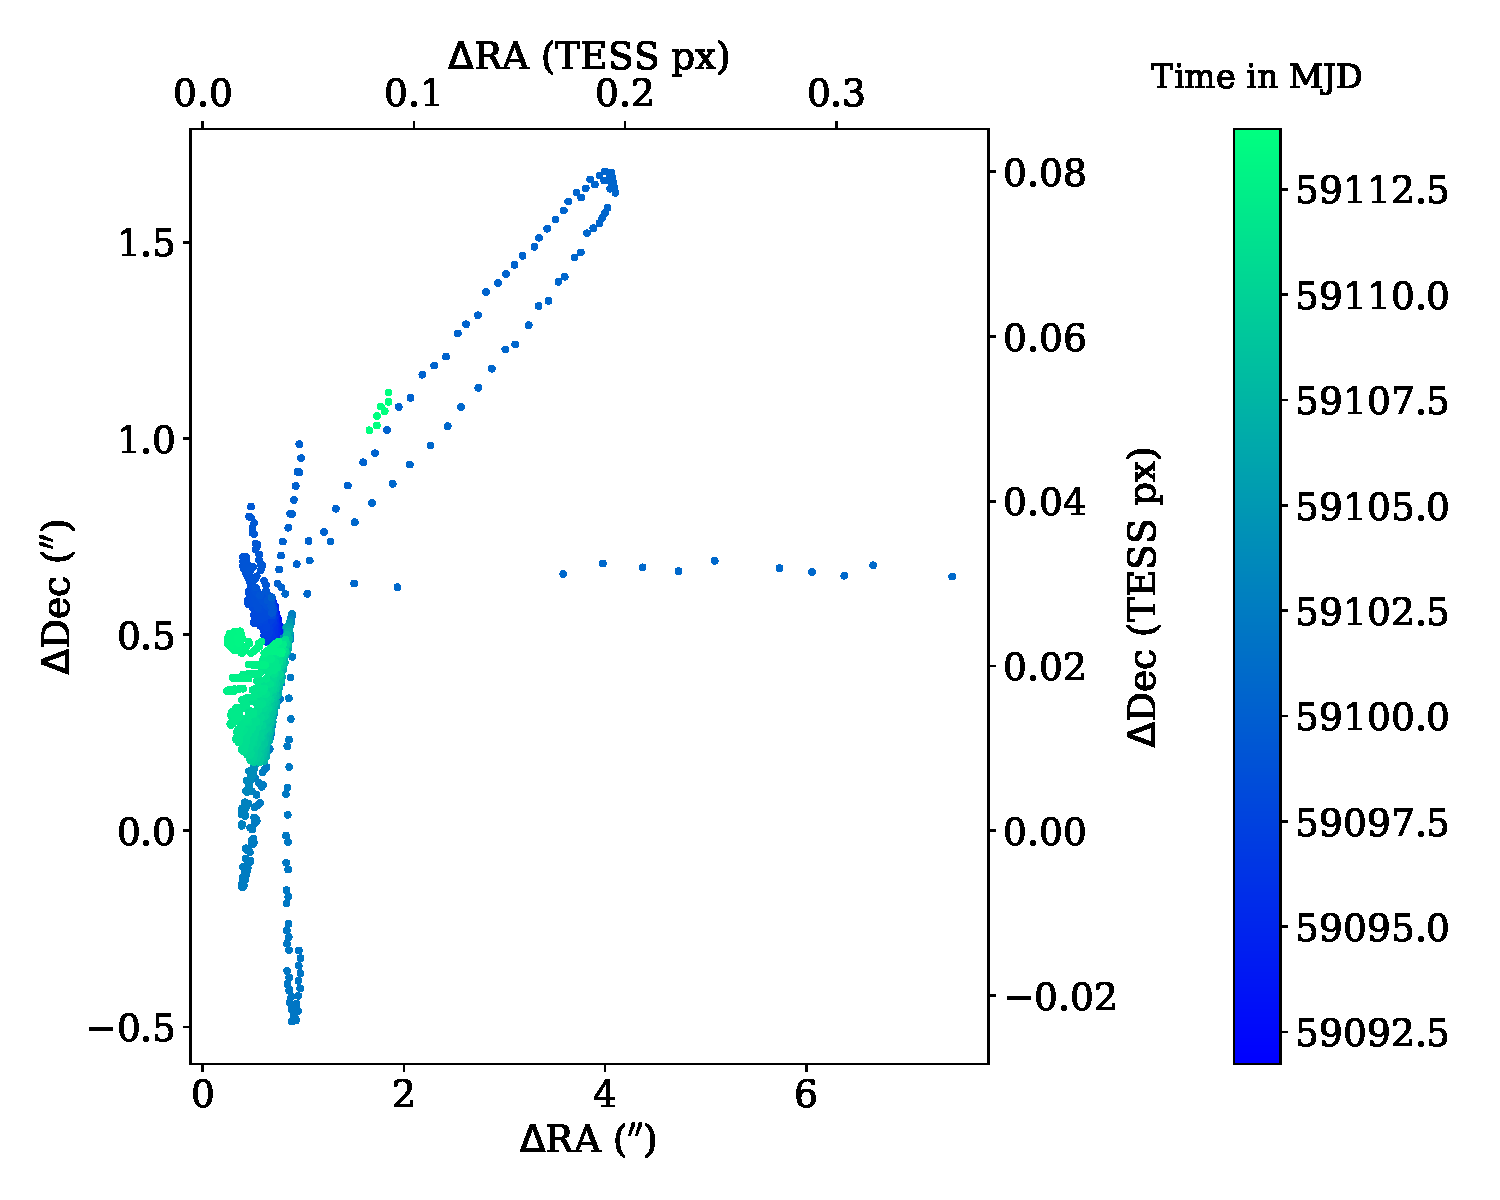
\includegraphics[width =0.8 \textwidth]{./Figures/1990 KC1PosCheck.pdf} %TODO one with more points???
  \caption[Interpolated Position Verification]{
    The difference in the interpolated position of an asteroid from queries to \texttt{JPL Horizons}.
    The change in position in both arcseconds (\unit{\arcsec}) and TESS pixels are shown.
  }\label{Fig:errPos}
\end{figure}

With TESS data coming in $\qty{10}{\minute}$ chunks, these positions are still very sparsely spaced in time compared to the TESS data.
72 interpolated points are needed between each \texttt{SkyBoT} query.
A linear interpolation between the queried RA and Dec is performed by \texttt{NumPy} \citep{Harris2020} at the times of the TESS frames.
\texttt{TESSELLATE} saves out these time-frame pairs as part of its analysis, allowing for the time coordinate of any position to be exactly at a frame time.
This will also simplify the detection matching, as the any difference in the time will mean the detection is in a different frame.

These interpolated positions can be seen in \autoref{Fig:interpPos} for a subsection of sector from \texttt{TESSELLATE}.
There are a few interesting features, such as the asteroids are moving in the same direction, indicated by the colouring with time.
They tend to decrease their RA and increase their Dec as the month of the sector progresses, generally moving from the bottom right to the top left of the figure.
There is also a large size range in this slice of sky, ranging over \qty{6}{\mag} in absolute magnitude, which can be seen in the alpha (or transparency) of the tracks in \autoref{Fig:interpPos}.

Because of a small change in position between each frame, \citep[$\sim \qty{1}{\px}$ per \qty{30}{min} FFI][]{Pal2018}, this interpolation should be accurate.
Checking this prediction against a higher frequency query to the \texttt{JPL Horizons} ephemeris confirmed this accuracy on a few asteroids, as shown in \autoref{Fig:errPos}.
This is of the asteroid (8654) 1990 KC1, but all other objects checked are just as accurate.
The largest difference is only a third of a TESS pixel in RA, so the interpolations are accurate enough for these measurements.

The high frequency queries are not a feasible way of getting the positions of all the asteroids.
The \texttt{JPL Horizons} queries are specific to the asteroid name and time of observation, so each asteroid needs as separate query for each TESS frame.
The cone search \texttt{SkyBoT} query would still be needed, to determine what asteroids are in the field to begin with.
All other objects checked with \texttt{Horizons} are similarly accurate to \autoref{Fig:errPos}, so it is also not needed for reliable positions.
The queries are also rate limited, so while a few asteroids can be checked, filling the gaps between the \texttt{SkyBoT} half day queries for all the asteroids would be too expensive.


\subsection{Matching Asteroids to \texttt{TESSELLATE} Detections}\label{SubSec:Match}

Matching these interpolated positions to \texttt{TESSELLATE} detections is important to lower the unknown transient outputs of this pipeline.
Taking previously unidentified detections and assigning them to an asteroid category, the remaining unknown transients can be more efficiently searched for other interesting astrophysical phenomena.
Having interpolated their positions, the asteroids have a well-sampled set of RA, Dec and time values of where they should be in the TESS data.
They should show up in a single pixel in $xy$ space for a few frames, of order $\sim1$.
This is the same as a lot of other transient events, a sharp rise in brightness and then disappearing quickly again.

The number of frames for events is variable \citep{TESSELLATE}.
For example, type Ia supernova will brighten is a matter of a few hours and then dim for days, while stellar flares are of a similar profile but have a smaller maximum brightness and a correspondingly shorter decay time.
Asteroids are very short events, however these detection pipelines are robust and do pick them up.
A goal of this work is to catch all the asteroids in the set of all the transients that are returned from the pipeline.
To achieve this, catalogue matching is in order.

Using the \texttt{KDTree} algorithm \citep{Maneewongvatana1999} as implemented in \texttt{SciPy} \citep{2020SciPy-NMeth}, the RA and Dec coordinates of the interpolated points and the detections can be compared and matched together.
Filtering this \texttt{KDTree} output by restricting the time between spatially coincident matches to less than \qty{0.1}{\day} stops any accidental matches in position from non-asteroid detections.
A cut is then made by distance, which must be smaller than \qty{0.01}{\degree} (\qty{36}{\arcsec}), which is within 1.7 TESS pixels.
Then, if multiple detections match the same interpolated point, the detection with the smallest distance to the match is taken.

An example of the matches found using this \texttt{KDTree} is shown in \autoref{Fig:RADecMatch}, and appear to be coinciding with the asteroid both spatially and temporally.
\texttt{TESSELLATE} is not detecting every frame that an asteroid is in.
Detections in \texttt{TESSELLATE} are done on a per-pixel basis, and asteroids only cross each pixel for a short number of frames.
The residuals of \autoref{Fig:RADecMatch} are all within a TESS pixel, shown on the right-hand axis of each of the lower panels.
The small residuals mean the filtering done after the \texttt{KDTree} was run worked as intended.

There are strings of frequently matched points, and then patches where there are few matches detected at all.
Not every interpolated point gets a match, due to a variety of reasons.
These all culminate in too small of a change in flux of the pixel from normal brightness and the frames where the asteroid is there.
The change has to be large for \texttt{TESSELLATE} to detect it, so only when the asteroid will only be matched when it is brightest.


\begin{figure}[]
  \centering
  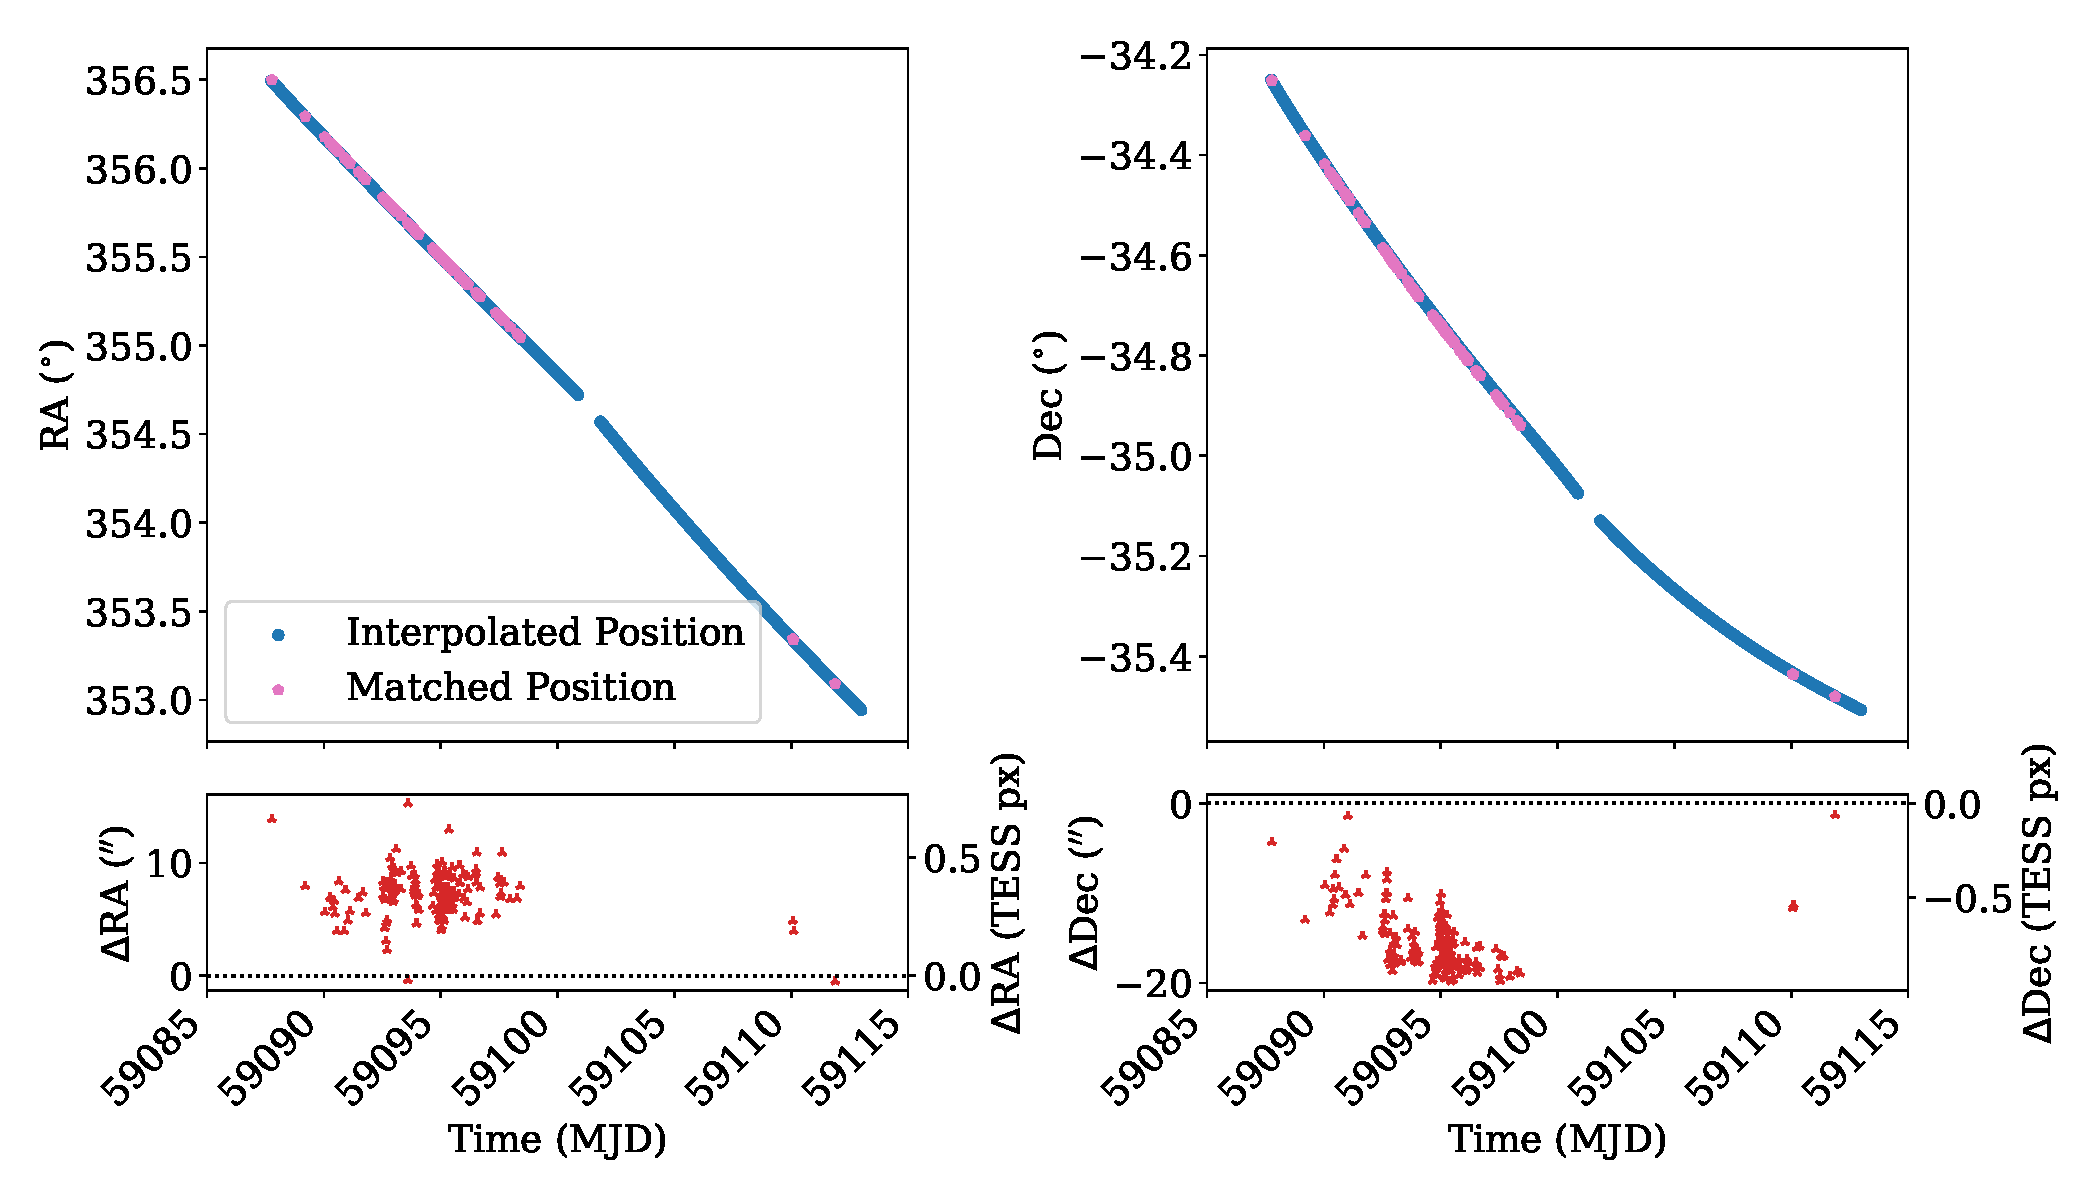
\includegraphics[width =\textwidth]{./Figures/DetectMatchPosUlysses.pdf}
  \caption[Interpolated and \texttt{TESSELLATE} Detected Positions Comparison]{The RA (right) and Dec (left) of interpolated position (blue dots) or the matches to \texttt{TESSELLATE} detections (pink hexagons) against the time of observation. The lower panels show the residuals of the difference between the positions for points that occur at the same time.}
  \label{Fig:RADecMatch}
\end{figure}

\subsection{Photometry and the Construction of Asteroid Lightcurves}\label{SubSec:Lightcurves}

%light curves; detected VS forced interpolated 
There are two sets of points to take light curves from.
The matches from the detections, which already have a flux calculated, and the interpolated points themselves, which are more numerous but require forcing the photometry.
\texttt{TESSELLATE} had already reduced all the FFIs using \texttt{TESSreduce}, I did not do any of the data reduction.

The flux for the forced photometry is calculated with \texttt{Photutils} \citep{Bradley2024} aperture photometry.
A \qty{1.5}{\px} radius aperture used, as this is the standard size used by the rest of \texttt{TESSELLATE}.
It is placed on the centre of mass (COM) position of a $5\times5$ \unit{\px} box around the integer $xy$ coordinate of the asteroid.
The COM was calculated using \texttt{Scipy} and the \texttt{ndimage.center\_of\_mass} routine.
The integer coordinates are found with the \texttt{SkyCoord} module of \texttt{Astropy}, the world coordinates, in RA and Dec, can be transformed into pixel coordinates, $x$ and $y$, using a world coordinates system (WCS) from \texttt{TESSELLATE}.

The integer coordinates from the interpolated positions were not used themselves because the asteroids seemed to be leading the object in any given frame of TESS.
This was decreasing the total flux of the asteroid, as the aperture  was hitting mostly background.
This also caused a ``sawtoothing'' effect, where the lightcurve would jump from a minimum to a maximum when the integer coordinate snapped from being a pixel out to back on the asteroid.

I did not take the highest pixel value in a box to correct this effect because there could be a rouge star in the field that it detects as the maximum, instead of the asteroid.
The COM technique would still be affected by such contamination, but the total change in position would be less.
The photometry on the COM aperture did fix the sawtoothing, as there is sub-pixel accuracy in the COM calculation.
There was a far smoother transition from maximum to minimum, as expected from rotating asteroids.
Hereafter, unless otherwise specified, ``flux'' refers to this COM flux measurement of the asteroid.

%TODO data cleaning explaination
A few steps need to be taken to clean these lightcurves.
Following \citet{McNeill2023}, any fluxes more than $3\sigma$ from the mean value are sigma-clipped recursively from the forced photometry lightcurves, until convergence is achieved.
The contamination from background stars the object passes is too great to allow in the lightcurve.
This does introduce gaps into an otherwise regularly sampled lightcurve, but this will not be a problem for the rotation period analysis.
Lightcurves with an average flux $<10$ counts are lost in the random noise floor, so a minimum mean flux limit needs to be applied to ensure quality and reliability of any periods calculated.

The subsections of the FFIs made by \texttt{TESSELLATE} have a small overlap.
If an object moves between these, there will be a few frames where it is found in multiple of these subsections.
This produces lightcurves that have two simultaneous observations of the asteroid, which clearly is not possible.
At the very edge of the subsections, the asteroid can have a position that would have the aperture be summing over pixels that are outside the field, and thus the asteroid would have a lower flux value on the edge.
The overlap is great enough that the decrease in flux should only be happening on one of the edges at a time.
By removing the duplicate observation times, keeping only those with the highest flux to filter out the edge cases, lightcurve is cleaned. 

\begin{figure}
  \centering
  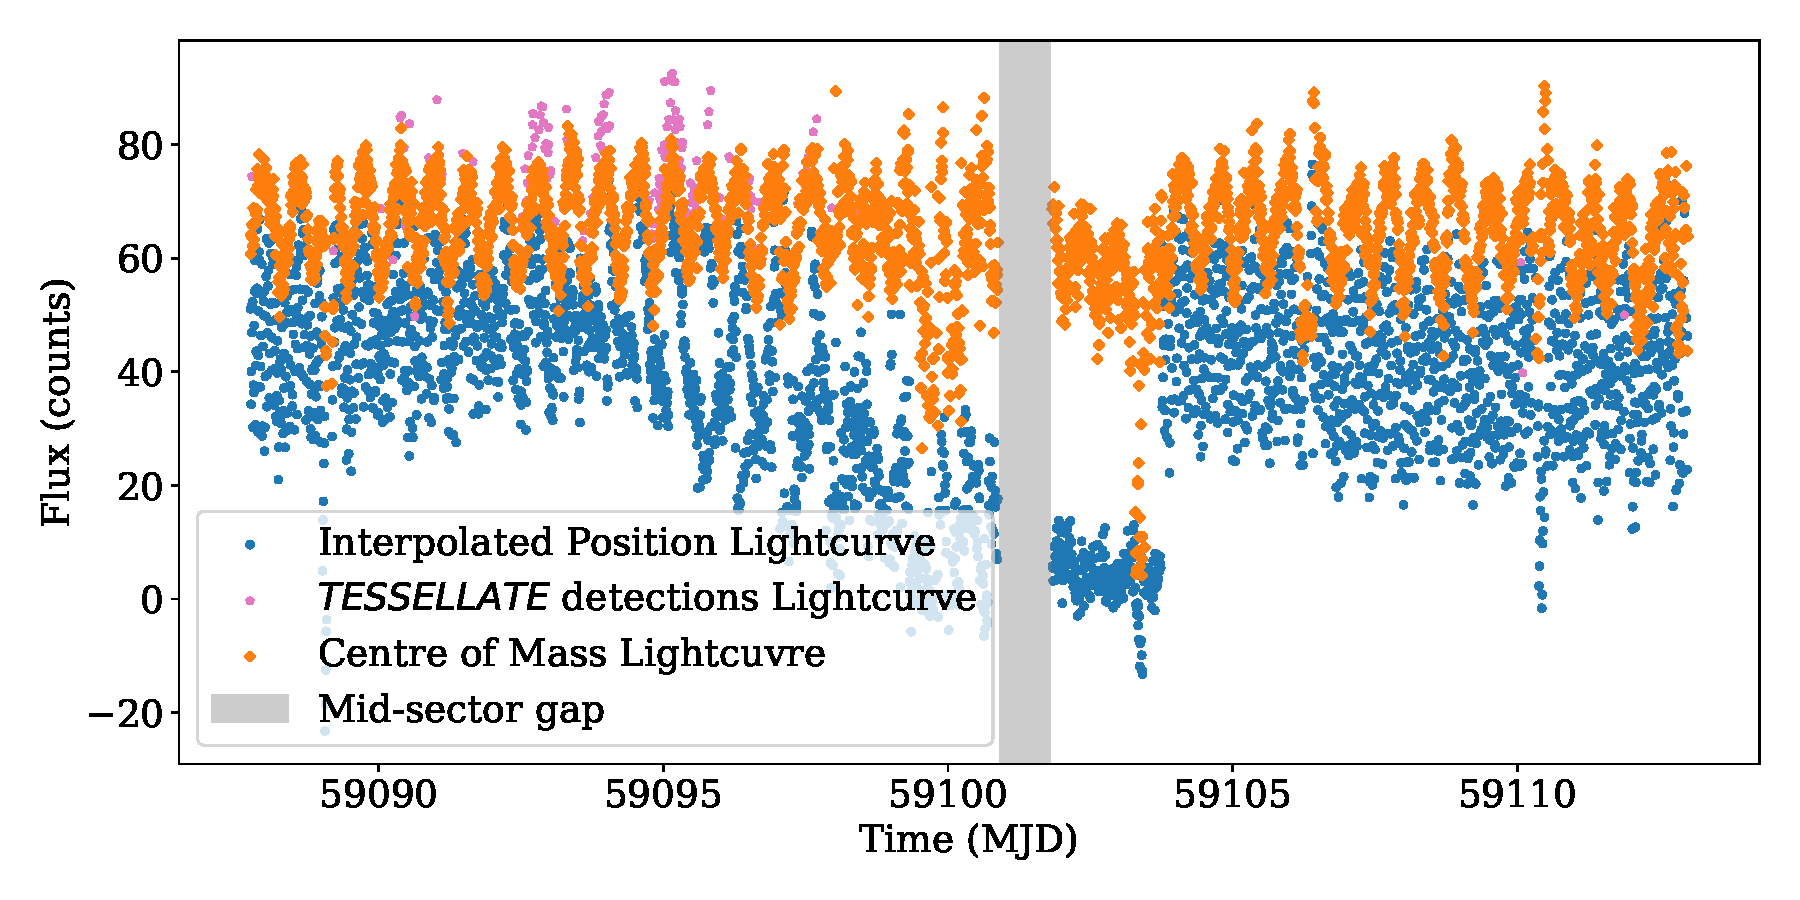
\includegraphics[width =\textwidth]{./Figures/SingleBodyLCUlyssesgapSpan.pdf}
  \caption[Lightcurve Example]{The light curves of the asteroid (5254) Ulysses throughout its entire journey across sector 29.
    The flux of the interpolated positions in blue circles, the \texttt{TESSELLATE} flux for any matched points in the pink hexagons, and the COM flux in orange diamonds.
    The mid-sector gap is highlighted by the grey shaded box.}
  \label{Fig:FullSingleLC}
\end{figure}

A comparison between the three light curves is interesting.
\autoref{Fig:FullSingleLC} shows these three light curves for a single asteroid, (5254) Ulysses.
The COM flux is much more stable than the interpolated positions flux, and has a higher average flux count.
This should result in a more accurate period analysis as there is less overall variation in the data caused by the misplaced aperture.
All the change in flux is instead due to the rotation of the asteroid.

The matched points are comparatively sparse for this object, as discussed above (\autoref{SubSec:Match}, \autoref{Fig:RADecMatch} is also (5254) Ulysses).
This is not the case for all asteroids.
Many have no matches, and some have almost fully matched.
The match rates for the sample in sector 29 will be discussed more later in \autoref{SubSec:Detect}.

\subsection{Calculation of Asteroid Rotation Periods}\label{SubSec:Periods}

%Periods and amplitueds for everything detected
The next part of my analysis involves determining the periods and amplitudes of each asteroid's light curve.
The rotation period and other properties of the lightcurve will be calculated from the forced photometry on the COM positions. 
The matching is still beneficial to the \texttt{TESSELLATE} pipeline as a whole, but is too sparse for this rotation analysis.

A widely used technique in determining the periods of astronomical data is the Lomb-Scargle periodogram \citep[\citet{Lomb1976,Scargle1982}, but see][for a review]{VanderPlas2018}.
This method can efficiently take discrete time-series data of which the observations are unevenly spaced and calculate the frequencies present in the sample.
TESS should have rather evenly spaced data, as the FFIs are produced on a set cadence, but sometimes data will be missing.
For example, it may have been sigma clipped due to a spike in brightness that is unphysical for an asteroid, or TESS sees the same asteroid in the same sector on either side of the day long mid-sector break it takes for data transfer.
The periodogram reduces to both a fast Fourier transform or a direct least squares fit in appropriate limits, but outperforms them markedly in unevenly sampled data \citep{VanderPlas2018}.

There are a few different implementations of a Lomb-Scargle periodogram available in world of astronomy python packages.
I have used the Lomb-Scargle periodogram as implemented by \texttt{Astropy}\citep[\citet{Astropy2022} but see][for the implementation]{Vanderplas2012,Vanderplas2015}.
The times are converted from days to seconds before the periodogram is calculated, so the frequency is calculated in \unit{\hertz}.
The flux values have their mean subtracted so the change in flux being analysed is about 0 counts.
\texttt{Astropy} has ways of doing this internally, but I opted to do it explicitly.

\texttt{Astropy} also returns a model, in the form of
\begin{equation}
  \label{Eq:LCModel}
  F(t;f,\vec{\theta}\,) = \theta_0 + \theta_1\cdot\sin{2\pi ft} +\theta_2\cdot\cos{2\pi ft}
\end{equation}
where the flux, $F$, is given in terms of time, $t$, the calculated frequency, $f$, and the model parameters $\vec{\theta} = [\theta_0, \theta_1,\theta_2]$.
These parameters are useful in reconstructing the model without rerunning the periodogram.
\texttt{Astropy} gives a statistic on how confident it is in the detected frequency is, the false alarm probability.

The chosen method used for the periodogram fits is the new \texttt{nifty-ls} package \citep{Garrison2024} that has can be implemented on its own, or by interfacing with \texttt{Astropy}.
I use the later implementation as the speed-up from the non-uniform fast Fourier transform is helpful.
The large dataset from \texttt{TESSELLATE} requires this calculation efficiency but the \texttt{Astropy} interface is how I was trialling my code on smaller datasets.

The minimum period returned by the periodograms will be set by the Nyquist limit of the data.
For the \qty{10}{\min} FFIs (the cadence analysed here), the Nyquist period is $\qty{20}{\min}=\frac13\unit{\hour}$, a threefold increase in time sensitivity from the longer FFIs
This will improve the sensitivity of TESS to fast rotating asteroids.
Based on their experimentation with the \qty{30}{\min} cadence FFIs, \citet{McNeill2023} find that periods less than \qty{3}{\hour} be interpreted with caution, due to lack of reliability in recovering injected sources.
Because of the increase in FFI rate, this time will be decreased to \qty{1}{\hour} for the minimum reliable period, as the lightcurve sampling on these timescales is equivalent.

A \qty{17}{\day} maximum period for periodogram analysis is recommended by \citeauthor{McNeill2023}.
If there is a lack of signal in the rotation curve, the calculated period to defaults this long period limit.
Such cases can be filtered out by keeping only periods less than \qty{90}{\percent} of this maximum, and removing all others from further analysis.

For the periodograms, I originally tried using the \texttt{Lightkurve} \citep{Lightkurve2018} package built for period analysis of TESS (and Kepler) data of variable stars.
There were interesting similarities and differences between the implementations.
\texttt{Lightkurve} was easy to use but did not allow for fine-tuning of the periodogram, or give any model of the best-fitting curve it produced.
\texttt{Lightkurve} is based on the \texttt{Astropy} methods, but does not give all the functionality, instead opting to simplify the process.

\begin{figure}[!t]
  \centering
  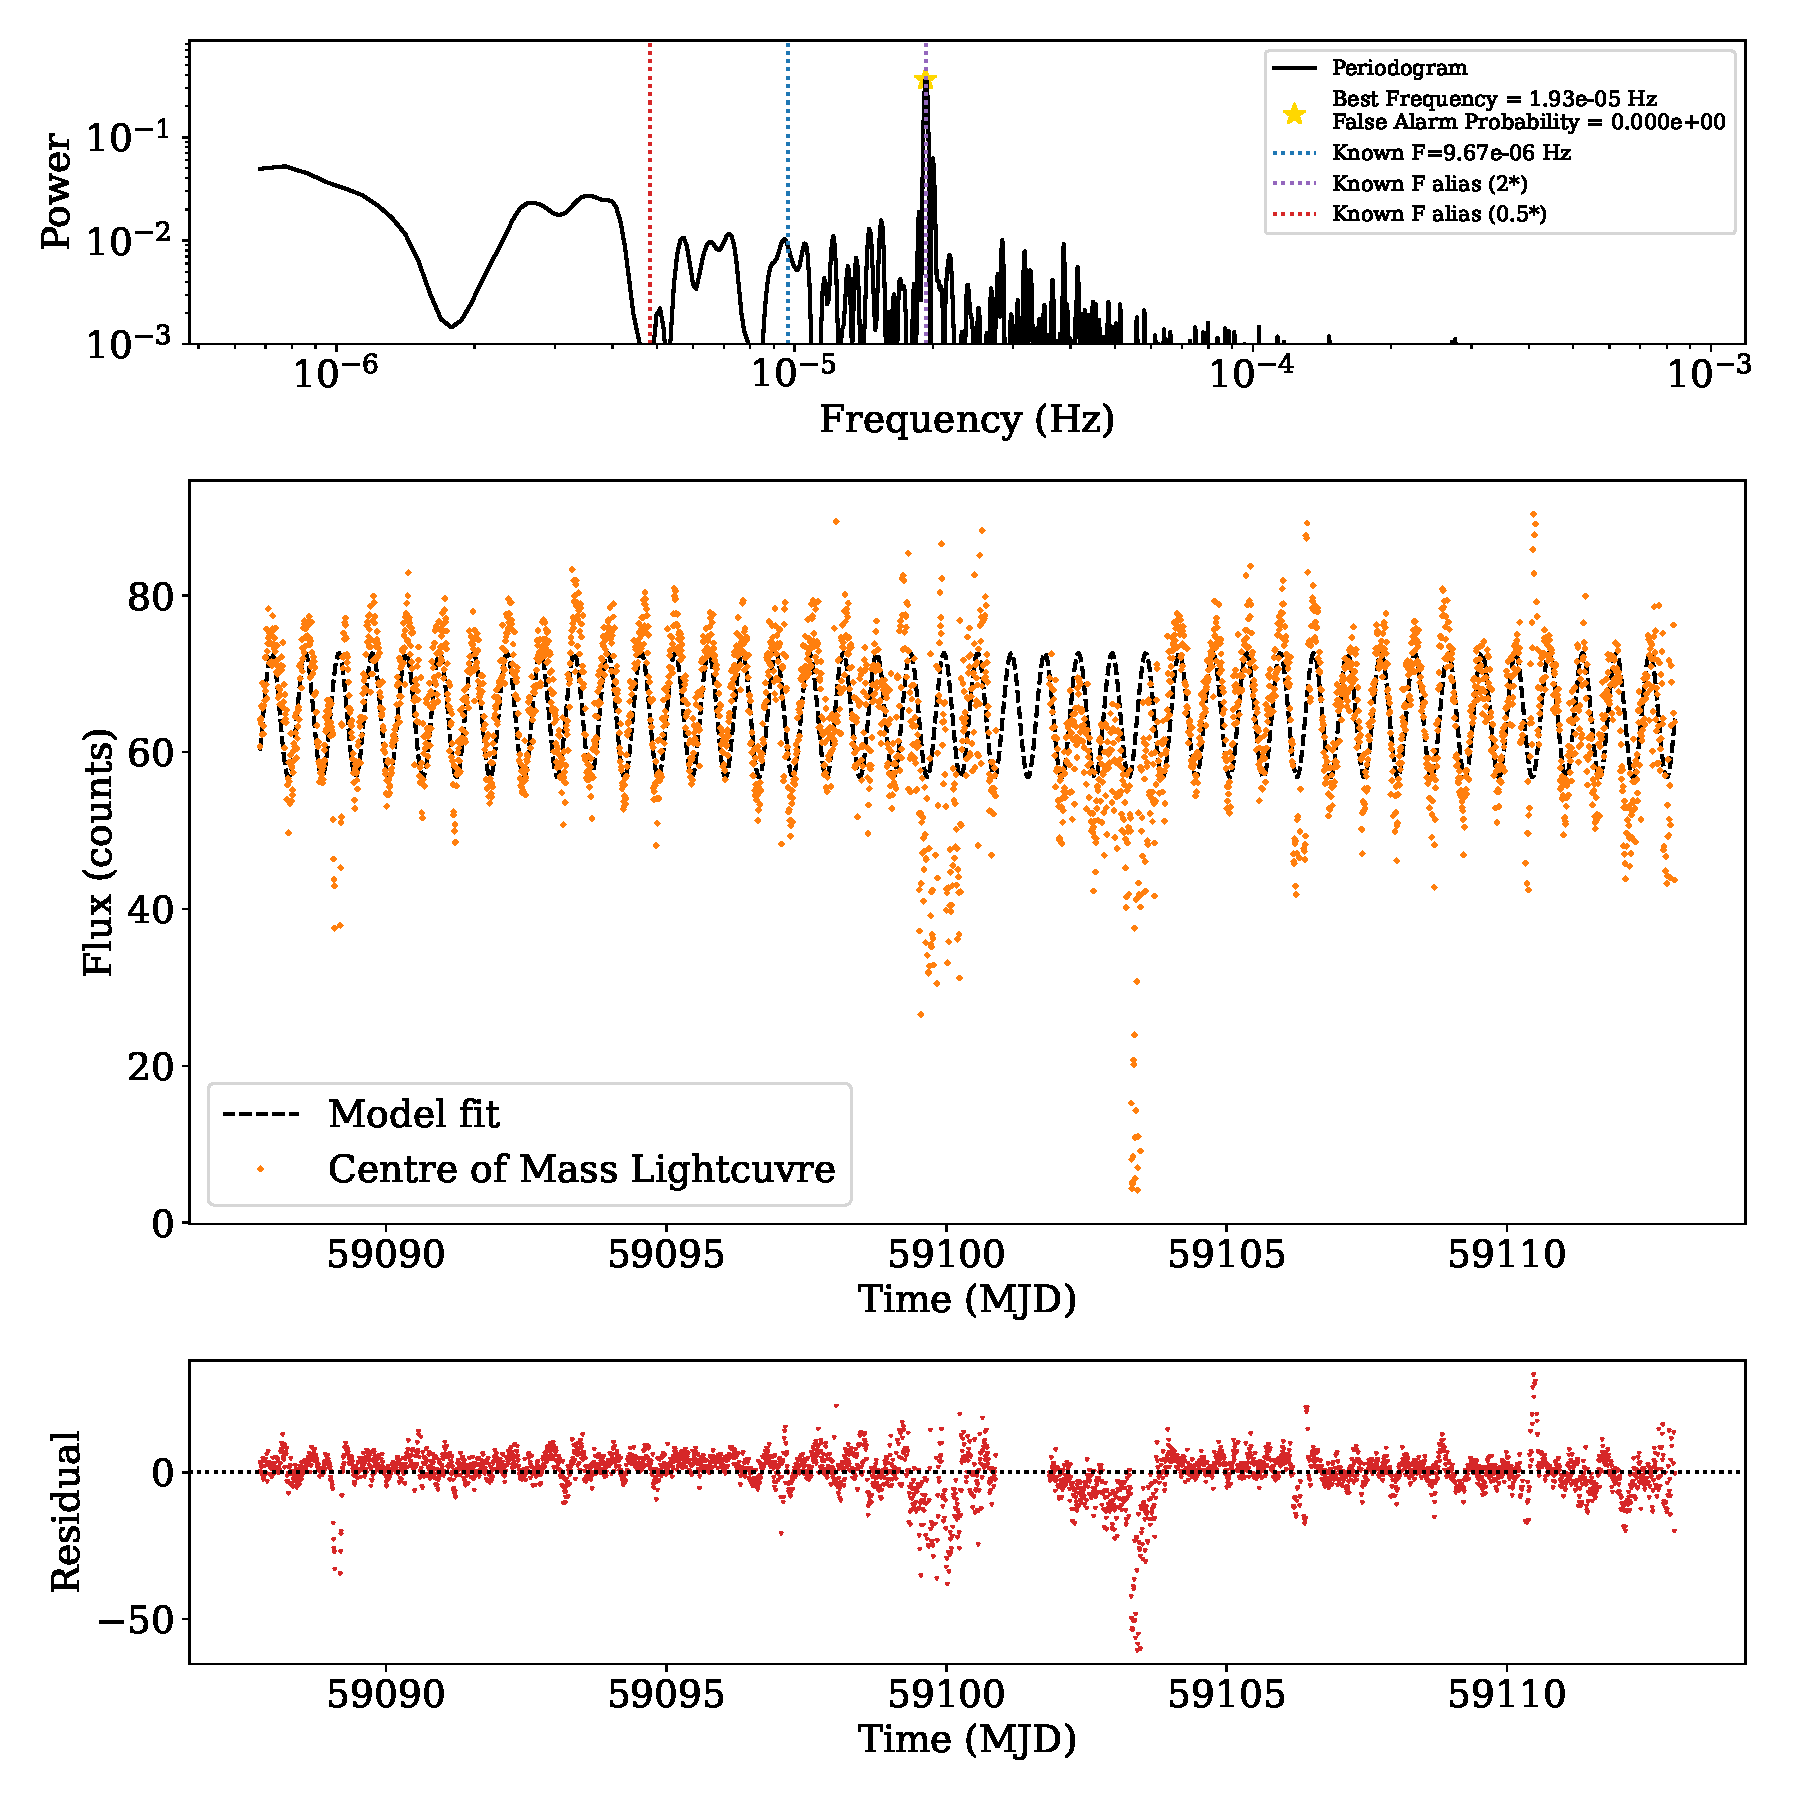
\includegraphics[width=\textwidth]{./Figures/PeriodogramUlyssesResid.pdf}
  \caption[Periodogram example]{\textit{Upper Panel}:The Periodogram of the COM flux of (5254) Ulysses.
    The maximum power of the periodogram is highlighted with the gold star.
    The known frequency, from the LCDB \citep{Warner2009}, is shown in the blue dotted lines, and a factor of 2 alias each way is shown in the purple dotted lines ($2*$) and red dotted lines ($0.5*$).
    \textit{Middle Panel}: The COM flux lightcurve and the returned model (dashed black curve) of the lightcurve from the periodogram analysis.
    The frequency of this model is the same as the gold stared point in the upper panel.
    \textit{Lower Panel}: The residuals of the model fit.
  }
  \label{Fig:PeriodEx}
\end{figure}


An example of such an \texttt{Astropy} Lomb-Scargle periodogram and the corresponding model fit to the lightcurve is given in \autoref{Fig:PeriodEx}, along with the residuals of the fit.
It is calculated that (5254) Ulysses had a frequency double that listed in the LCDB, as seen with the vertical dotted lines.
This is expected due to the double-peaked nature of most asteroid lightcurves \citep{McNeill2023}.
This asteroid was highlighted as an alias of the known frequency is recovered by this analysis.
To account for this, the detected periods will be doubled to obtain the true rotation period of the object.

The peak highlighted with a gold star in \autoref{Fig:PeriodEx} is the most prominent peak in the periodogram.
The periodogram is limited below at a power of $10^{-3}$ to highlight only the regions with large power.
Not all the asteroids have such well-defined maximums, and the peak power of the periodogram is an important factor in its quality.
A peak power less than 0.1 means there is little to no signal observed, and it will be almost indistinguishable from the noise.

The middle panel of \autoref{Fig:PeriodEx} shows the model given in \autoref{Eq:LCModel} fit to the COM flux lightcurve by \texttt{Astropy}.
This looks to be a good fit, with the peaks and troughs lining up.
The amplitude of the sinusoid appears to be slightly lower than the variation of the data, but it is consistent with the scatter.
This model is successfully fit over the mid-sector break in the lightcurve, and ignores the observations with a lower flux that did not quite get sigma clipped as they are within $3\sigma$ of the mean flux.

The lower panel in \autoref{Fig:PeriodEx} shows the residuals of the model subtracted from the data.
For the majority of the observations, the residuals are close to the 0 line, indicating a high quality fit.
There are places where there is a significant deviation from 0, corresponding to places in the lightcurve that look out of place to the eye.
These large residuals could be removed by decreasing the tolerance on the sigma clipping, but that could cut true signal in lightcurves with a large variation amplitude.

The amplitude of the variation is calculated from this model fit.
This is measured in magnitudes, and as such is found from the standard
\begin{equation} \label{Eq:DelMag}
  \Delta m = -2.5 \log_{10}(\frac{F_{min}}{F_{max}})
\end{equation}
with $\Delta m$ being the variation amplitude.
The $F_{min}$ and $F_{max}$ terms in \autoref{Eq:DelMag} and the minimum and maximum flux of the model, respectively.
These are measured in counts.




\subsection{Periodogram Quality Checks}\label{SubSec:QualCheck}

For accurate statistics, reliable data is needed.
So there must be checks on the quality of the values calculated.
Some of these have been discussed already, but for completeness I list them again here.
A lightcurve must have a mean flux of at least 10 counts to be reliable.
For an accurate periodogram, it is required that the lightcurve also contain more than 200 observations.
This is very easy for TESS and its \qty{10}{\minute} cadence, as the asteroid only has to be in the sector for \qty{33.3}{\hour}.
The periodogram itself must have a peak power of at least 0.1 to be distinguished from the noise
The calculated period must be $\qty{1}{\hour}\leq P \leq \qty{367.2}{\hour}$, where the upper bound is \qty{90}{\percent} of the \qty{17}{\day} window suggested by \cite{McNeill2023} is taken from their recommendation and adjusted for the shorter FFI times.


\section{Results}\label{Sec:Res}

Here I present the results for TESS sector 29.
Similar analysis can be preformed, and the same figures made, for any of the sectors.
The computation time was a limiting factor in getting more sectors processed.
There were 5664 objects detected in the sector with $V\leq \qty{20}{\mag}$, of which 374 passed all the quality checks imposed on their lightcurve and periodogram.


\subsection{Quality Check Verification}\label{SubSec:QualCheckVer}

\begin{figure}[t]
  \centering
  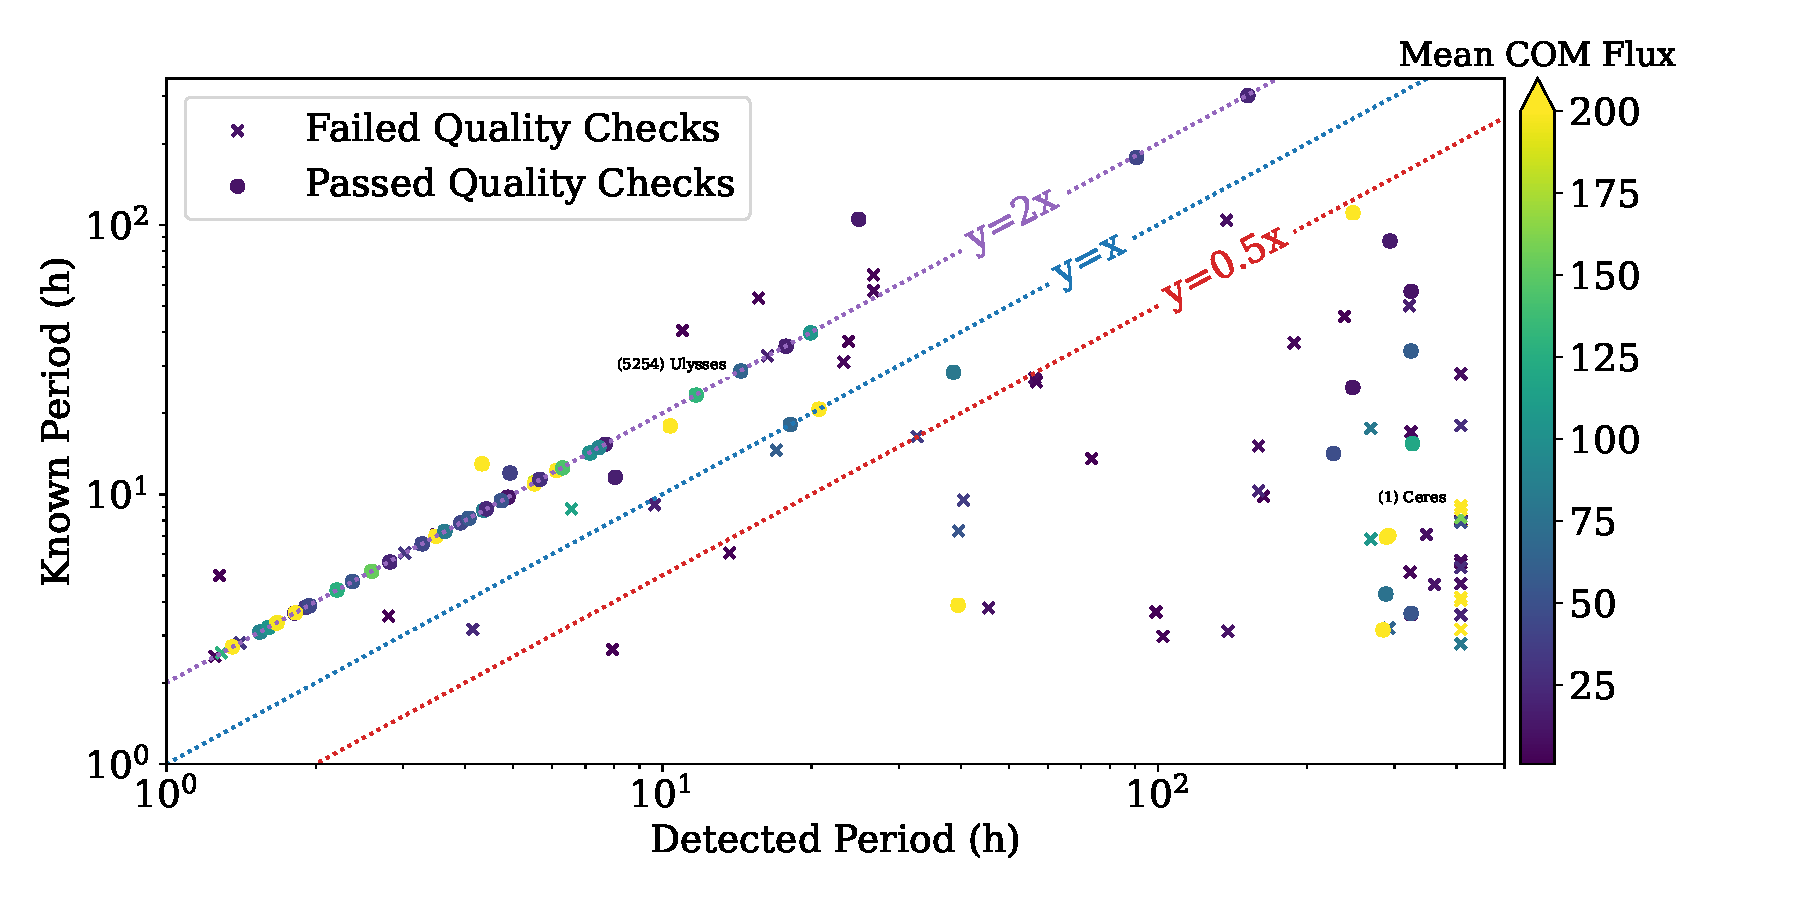
\includegraphics[width=\textwidth]{./Figures/LCBDcompFinal.pdf}
  \caption[Detected Period Compared to Known Period (LCDB)]{A comparison of the detected periods of the objects in the sector to their known periods in the LCDB \citep{Warner2009}, coloured by the mean flux of the object.
    Crosses failed the quality checks, while circles passed them.
    Names of asteroids are referring to the data point to the right of the text.
    Dotted lines of a constant relationship are plotted, coloured to show the same relationship to the known value as \autoref{Fig:PeriodEx}.
  }
  \label{Fig:LCDBcomp}
\end{figure}

While some quality checks were chosen to agree with the past work of others, some were chosen to make sure the derived periods were in agreement with the known ones from the LCDB.
A comparison between objects in both the sector and the LCDB is seen in \autoref{Fig:LCDBcomp}.
Of the 121 objects in both samples, 59 of them passed all the checks.
These are included in the total 374 asteroids that pass  all the quality checks in sector 29.
This means over \qty{80}{\percent} of the asteroids that pass all the checks do not have known periods.
The periods plotted are the output of the periodogram, they have not yet been doubled to account for the double-peaked lightcurve.

\autoref{Fig:LCDBcomp} is coloured by the flux of the asteroid to give an idea of what quality check the object failed.
If a cross is bright yellow, the periodogram checks would have been responsible, as the average flux is well above the necessary 10 counts.
The one bright asteroid that failed the checks in the top left is on the boundary of the \qty{1}{\hour} lower limit, indicating that this bound may be slightly too lenient.
The vertical line of crosses on the right-hand side of \autoref{Fig:LCDBcomp} highlights the maximum window of searched periods at $\qty{408}{\hour}$, and demonstrates why the \qty{90}{\percent} upper bound is necessary.
Many asteroids, across an order of magnitude of known periods and across the range of mean fluxes, have detected periods at the edge of the window, showing that the periodogram will return this value when no signal is present.

The largest asteroid, (1) Ceres, is highlighted in \autoref{Fig:LCDBcomp}.
It is not recovered, as it is almost too bright for TESS, and the flux bleeds into too many pixels for a rotation period to be accurately obtained from the \qty{1.5}{\px} aperture used.
An exception to the methods is not made here, and no reanalysis is attempted.
However, the periodogram and lightcurve are given in the appendix, \autoref{ApFig:Ceres}.
This object is the main reason for the arrow on the colour bar indicating higher mean flux values without a change in colour.
(1) Ceres has a mean flux is over 150000 counts which, if included, completely washes out the gradient.
200 counts was chosen as a replacement value because of the range of detail that can be identified.

The brightness of those asteroids that passed the checks is also useful to see.
If a circle is dark blue, it may only just be above the minimum requirements for average flux.
A range of brightness pass the checks, indicating sensitivity to a wide range of distances and sizes.
These are the two competing effects that determine the average flux of an object, those that are further away need to be larger to reflect the same amount of light to the detector.

The yellow circles in the lower right of \autoref{Fig:LCDBcomp} are cause for concern, as these are bright asteroids that are passing the checks with an incorrect period.
There are a dozen asteroids that pass the checks with large detected periods when compared to their known period.
These points imply the checks are not perfect.
Some experimentation was done on the limiting values, and the ones presented here achieved the highest recovery of accurate asteroid periods, while minimising the number that were incorrectly recovered.

The $y=2x$ line of \autoref{Fig:LCDBcomp} is of interest here, the known periods being twice the detected period.
This line corresponds to the calculated frequency being an alias of double the known frequency, as frequency and period are inverses of each other.
This is expected, the periodogram should return values on this line due to double-peaked lightcurves.
As seen in \autoref{Fig:PeriodEx}, (5254) Ulysses falls on this line, highlighted by text in \autoref{Fig:LCDBcomp}.
Most of the asteroids the pass the cut line along or near this key relation.
Few asteroids on the line fail the checks, which is also reassuring that the checks do what they are supposed to and filter out incorrect periods.

The idea of doubling the detected period was called into question due to the two of points recovered nicely on the $y=x$ line, indicating that the true period is found.
Either the LCDB has not accounted for the alias,  or the rotation signal sometimes returns the true period.
The former is unlikely as I only took the periods with high quality codes as recommended by \citet{Warner2009}.
The latter implies the lightcurve is not double-peaked, as is normally expected.
On the whole, there are enough periods that pass the checks with incorrect periods that these extra erroneous periods will not significantly change the fraction of reliable detections.

In total, 18 asteroids have periods that are not compatible with the LCDB.
With the 59 objects that pass the quality checks, this means \qty{70}{\percent} of the rotation periods calculated are accurate.
Including those periods that find a different alias of the rotation rate, falling near the $y=x$ or $y=0.5x$ lines, this value only increase to \qty{75}{\percent}. 
Considering that the detected periods are doubled to obtain the rotation period, the \qty{70}{\percent} accuracy is a better reflection of the data.  


\subsection{Asteroid Properties}\label{SubSec:AstPropRes} %TODO fix name

A plot of the semi-major axis against the other proper elements, eccentricity and inclination, is shown in \autoref{Fig:AEI}.
Looking at the data as a whole, all objects in the field of the instrument during the sector, with $V \leq \qty{20}{\mag}$, are plotted.
The exception being centaurs, which have an $a$ too larger for the detail in the distribution of the majority of the objects to be seen, and comets, which have an undefined $a$.
Shown in green dots, the 374 objects that passed all the quality checks have a similar distribution of orbital parameters to the total sample of 5664 small bodies in the sector.
This shows just how beneficial TESS is, and why its full sky coverage is so important to solar system science.

The distinction between the resonances in the main belt can be seen in \autoref{Fig:AEI}.
There are vertical strips separating the middle belt from the inner and outer belt.
The Jupiter Trojans are well-defined, at just past \qty{5}{\au}, with a small range of eccentricity but a large spread in the inclination.
A some Mars crossers and near earth asteroids (NEAs) at progressively smaller $a$ and a few more objects that are scattered with high $e$ and/or $i$ complete the distribution.

\begin{figure}
  \centering
  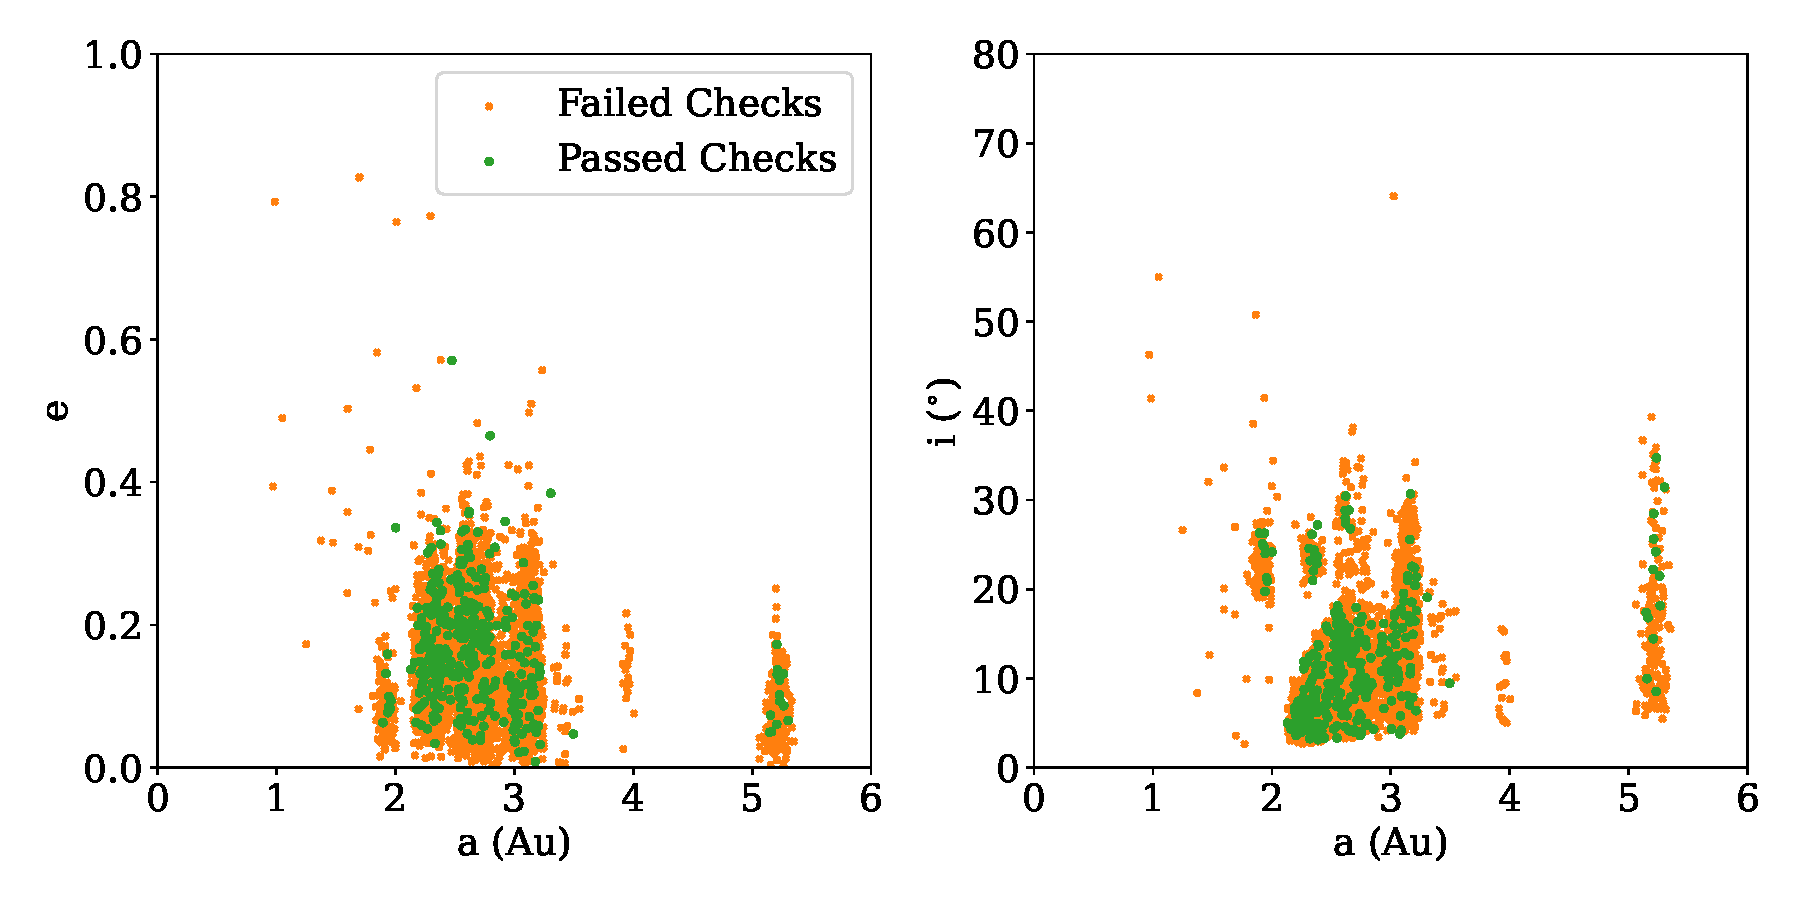
\includegraphics[width=\textwidth]{./Figures/AEIplotqualCut.pdf}
  \caption[Proper Element Distribution]{
    The $a$ against both $e$ and $i$ of the objects that \texttt{SkyBoT} found in Sector 29 with $V <\qty{20}{\mag}$.
    The orange crosses are those objects that did not pass the quality checks on the lightcurve and periodogram, while the green is those that did.
    The values of these proper elements were queried from \texttt{JPL Horizons} on 30/09/24.
  }
  \label{Fig:AEI}
\end{figure}

The number of asteroids belonging to each class of objects is highlighted in \autoref{Fig:NumPerClass}.
As expected from the orbital elements in \autoref{Fig:AEI}, the majority of the minor planets fall in the three regions of the main belt.
There are some objects that are not asteroids, 20 comets were in the field, along with one centaur.
While they have a V \unit{\mag} less than 20, these objects are not bright enough to have lightcurves with high enough mean fluxes to be detected well by TESS. 
As seen by the green bars in \autoref{Fig:NumPerClass}, around \qty{5}{\percent} of any class have lightcurves and periodograms that pass the quality checks, and this is relatively class independent.
The highest fraction is the detection of one object in the Amor family of NEAs.
However, with only nine total objects in the dataset, the sample is too small to make claims on the detectability of this class as a whole.

\begin{figure}
  \centering
  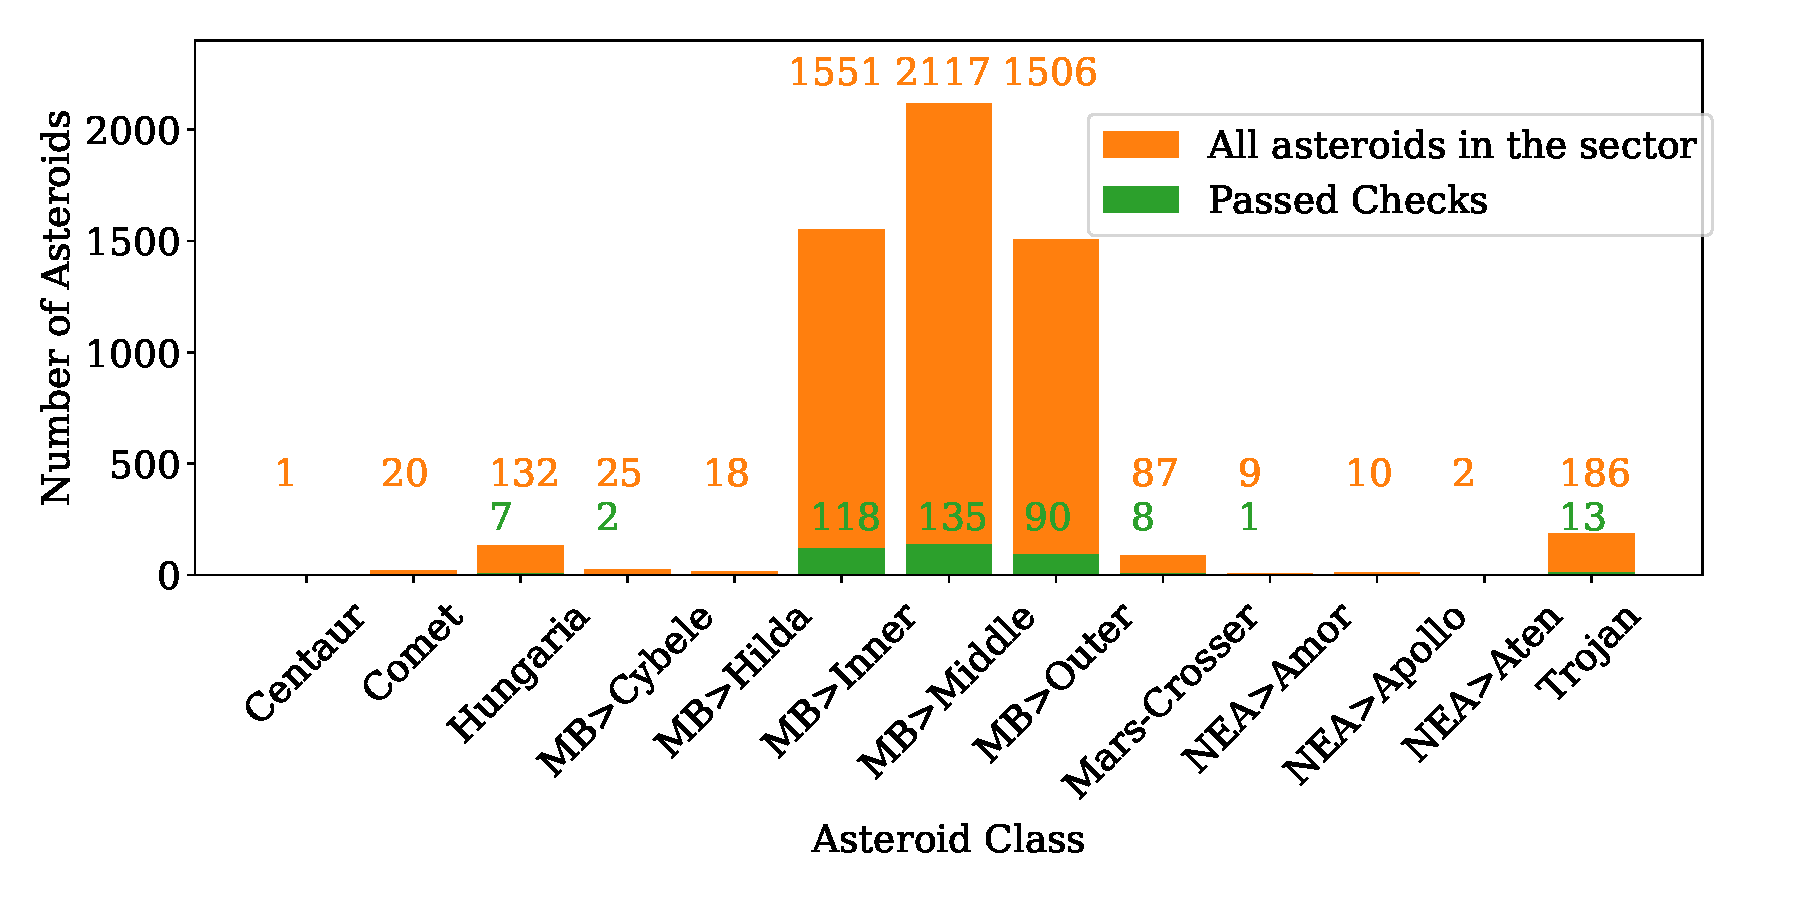
\includegraphics[width=\textwidth]{./Figures/classesBarqualCut.pdf}
  \caption[Asteroid Class Distribution]{A bar chart distribution of the total number of objects per class that \texttt{SkyBoT} found in the Sector (orange) and the same distribution of those that passed all the quality checks (green).
    The numbers above each class (coloured the same) correspond to the height of the bar, as some classes have too few objects to be seen.
    As with \autoref{Fig:AEI}, this is for all objects brighter than \nth{20}\unit{\mag}.
    For the class labels, MB is ``main belt'' and ``NEA'' is near earth asteroid.}
  \label{Fig:NumPerClass}
\end{figure}

\subsection{Asteroid Detectability in TESS} \label{SubSec:Detect}

\begin{figure}
  \centering
  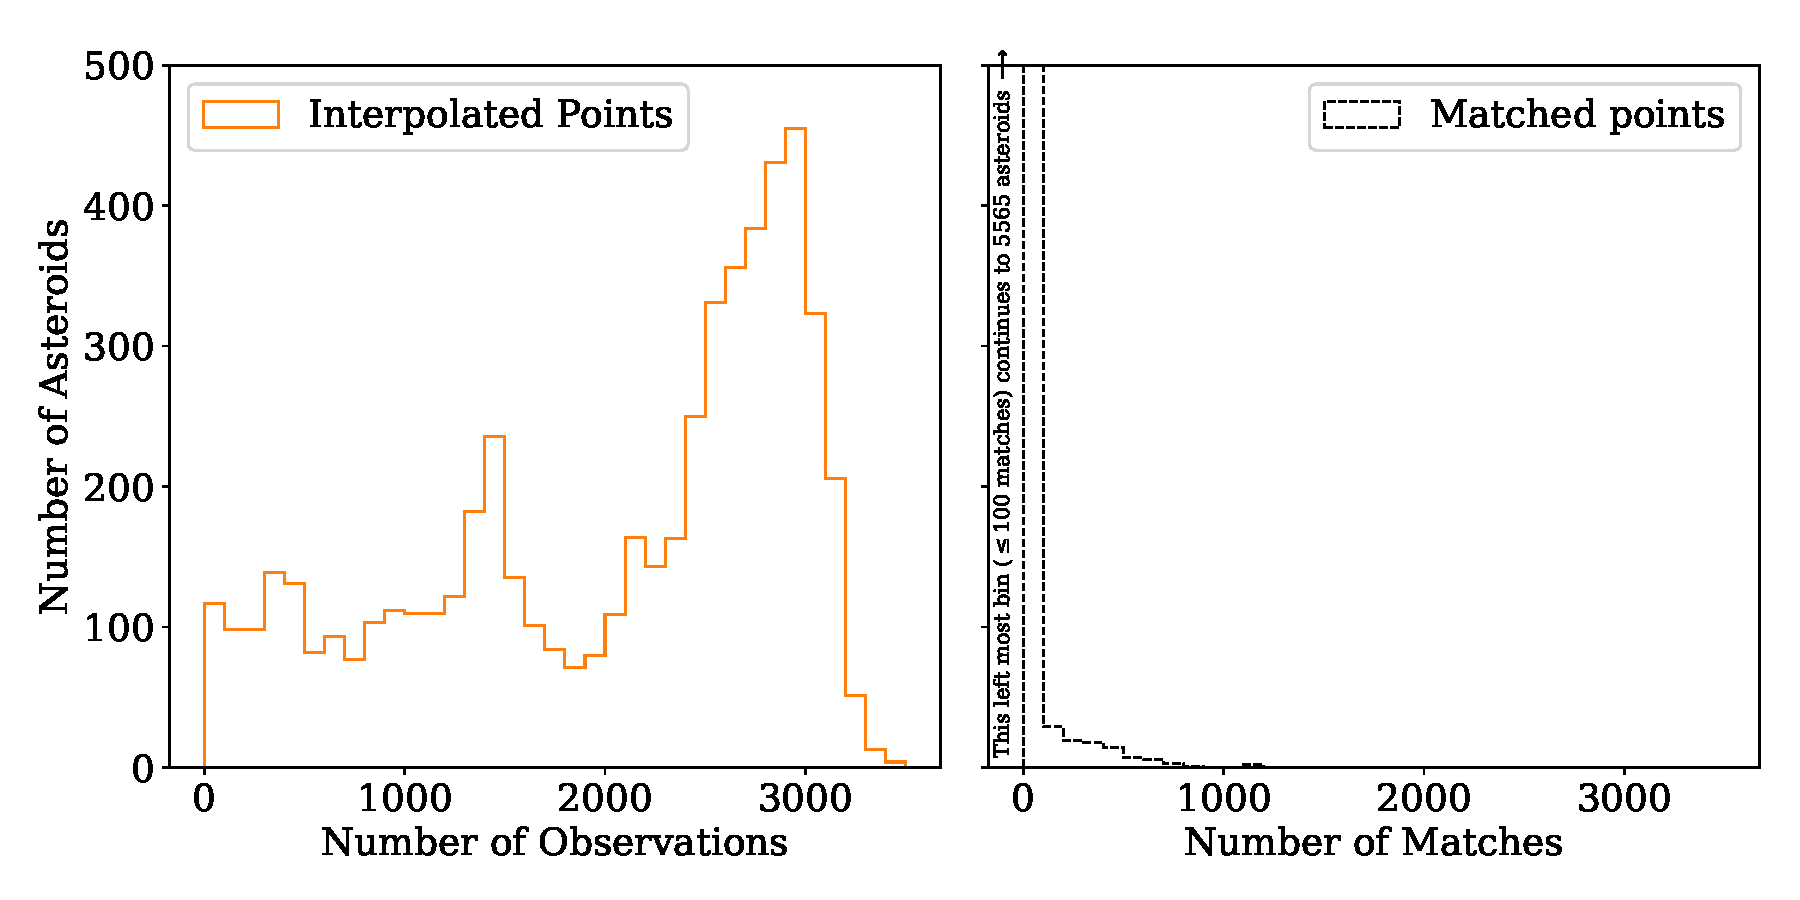
\includegraphics[width=\textwidth]{./Figures/pointsMatchesNumberHistdoubleChangedbound.pdf}
  \caption[Observation and Match Number Distribution]{\textit{Left}: A histogram of the number of observations in the lightcurve of each asteroid (orange solid line) in 100 observation bins. \textit{Right}: The number of matches each asteroid gets in the \texttt{TESSELLATE} detections (black dashed).
  }
  \label{Fig:MatchInterpHists}
\end{figure}

The number of forced photometry observations in a lightcurve is more evenly distributed than the number of matches, as shown in \autoref{Fig:MatchInterpHists}.
The quality cut of 200 observations in a lightcurve only cuts out $\sim 200$ asteroids.
Most asteroids are well sampled, with the mode of the distribution in the 2900 to 3000 observation bin, which means most of the asteroids are in a large fraction of the  $\sim3500$ frames in a sector of this cadence.

The matches have a very different distribution to the observations.
While both plots are limited to 500 asteroids on the y-axis, the matches' histogram in the right plot far exceeds this in the first bin, $\leq$ 100 matches, as indicated by the text and arrow.
Yet the y-limit is too large for detail to be seen in any higher bin of this plot.
There are only a total of 99 asteroids, out of the 5664 in the sector, that are matched more than 100 times to \texttt{TESSELLATE} detections.
So using the matches as lightcurves for periodogram analysis would mean most fail the minimum observations check, which limits the sample before any periods are calculated.

\begin{figure}
  \centering
  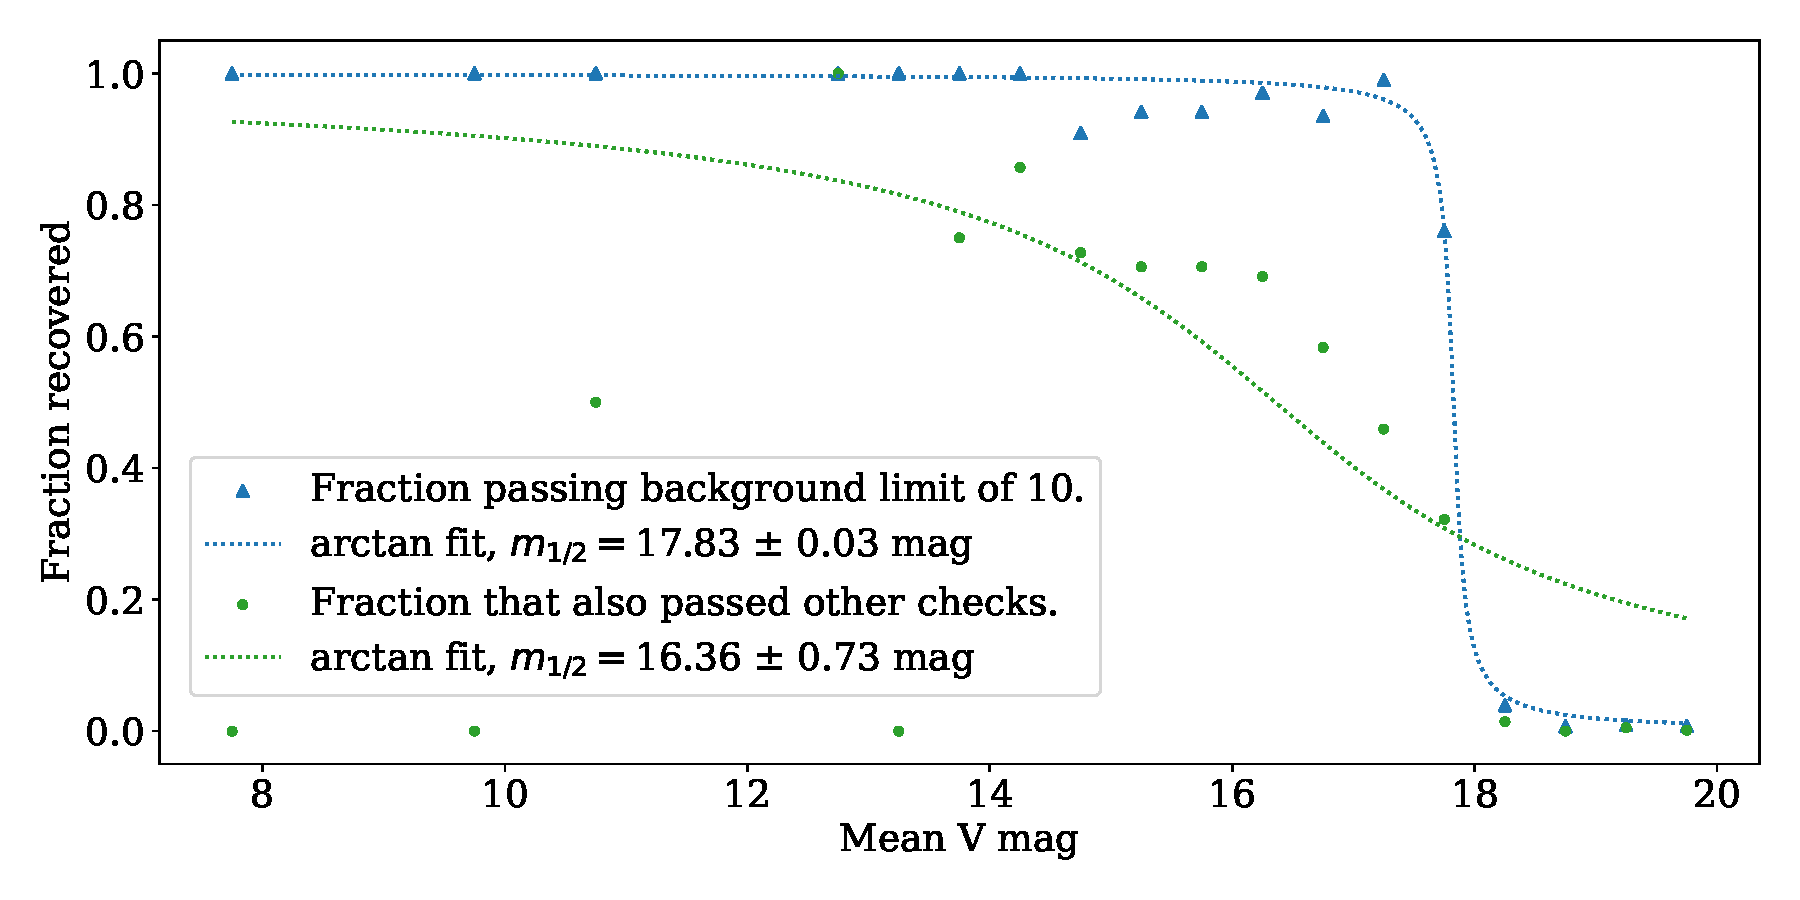
\includegraphics[width=\textwidth]{./Figures/recoverdHistBkgLimof10AtanBothLegendFixed.pdf}
  \caption[Visual Magnitude Recovery]{The recovery fraction against the known visual magnitude of each object in \qty{0.25}{\mag} bins.
    Coloured by whether the object exceeds only the mean flux requirement of the quality checks (blue triangles) or passes all the quality checks on the lightcurve and periodogram (green circles).
    A fit of an $\arctan$ function is provided in dotted lines of the same colour.
  }
  \label{Fig:RecovPassorFail}
\end{figure}

It is clear for \autoref{Fig:RecovPassorFail} that the mean flux check prohibits most of the asteroids dimmer than \nth{18} \unit{\mag}  from being detected.
The other checks cut down in the middle of the brightness range of objects rather evenly.
The brightest bins are not reliable data points because they only have a few asteroids in them. The values they can take on are too discrete.
(1) Ceres has $V<\qty{8}{\mag}$ and is not recovered, as discussed in \autoref{SubSec:QualCheckVer}, and is the only object in this magnitude bin, so a recovery fraction of 0 is returned.


The fits of to the fraction recovered in \autoref{Fig:RecovPassorFail} take the form
\begin{equation} \label{Eq:Atan}
  y= 0.5 -\frac{1}{\pi} \arctan(\alpha \cdot (m-m_{1/2}))
\end{equation}
where $y$ is the recovered fraction, $\alpha$ is how the steep the transition from 1 down to 0 is,  $m$ the magnitude and $m_{1/2}$ is the shift along the magnitude axis.
The constant of 0.5 in \autoref{Eq:Atan} raises the point of inflection to be at $\frac12$, and the $\frac{-1}{\pi}$ forces the range of the function to between the expected maximum at bright magnitudes at \qty{100}{\percent} recovered, down to \qty{0}{\percent} when dim asteroids are not detected.
The $m_{1/2}$ parameter dictates the limiting magnitude, as dimmer than this value less than half of the asteroids are recovered.
The fit is preformed on all bins (of \qty{0.5}{\mag}) dimmer than the first bin with more than one asteroid in it, to stop the discrete values from extremely bright asteroids from having too much influence.

There is a significant change in $m_{1/2}$ between the recovery curves in \autoref{Fig:RecovPassorFail}.
When only the minimum average flux of 10 counts requirement is applied, the limiting magnitude is $m_{1/2}= \qty{17.83(0.03)}{\mag}$.
When all the quality checks are imposed, this gets over a \unit{\mag} brighter, to \qty{16.36(0.73)}{\mag}.
It is expected that a higher threshold for quality will make the limiting magnitude brighter.
The $m_{1/2}$ for those that pass the full suite of quality checks is rather uncertain because of the scatter in the recovery fraction at brighter magnitudes.
The shallower decrease in efficiency also affects the uncertainty.
As it is no longer strictly a brightness cut-off that is being imposed on the data, the recovery fraction does not quite follow the $\arctan$ shape.


\subsection{Rotation Period Analysis Results}\label{SubSec:PerRes}


\begin{figure}[!b]
  \centering
  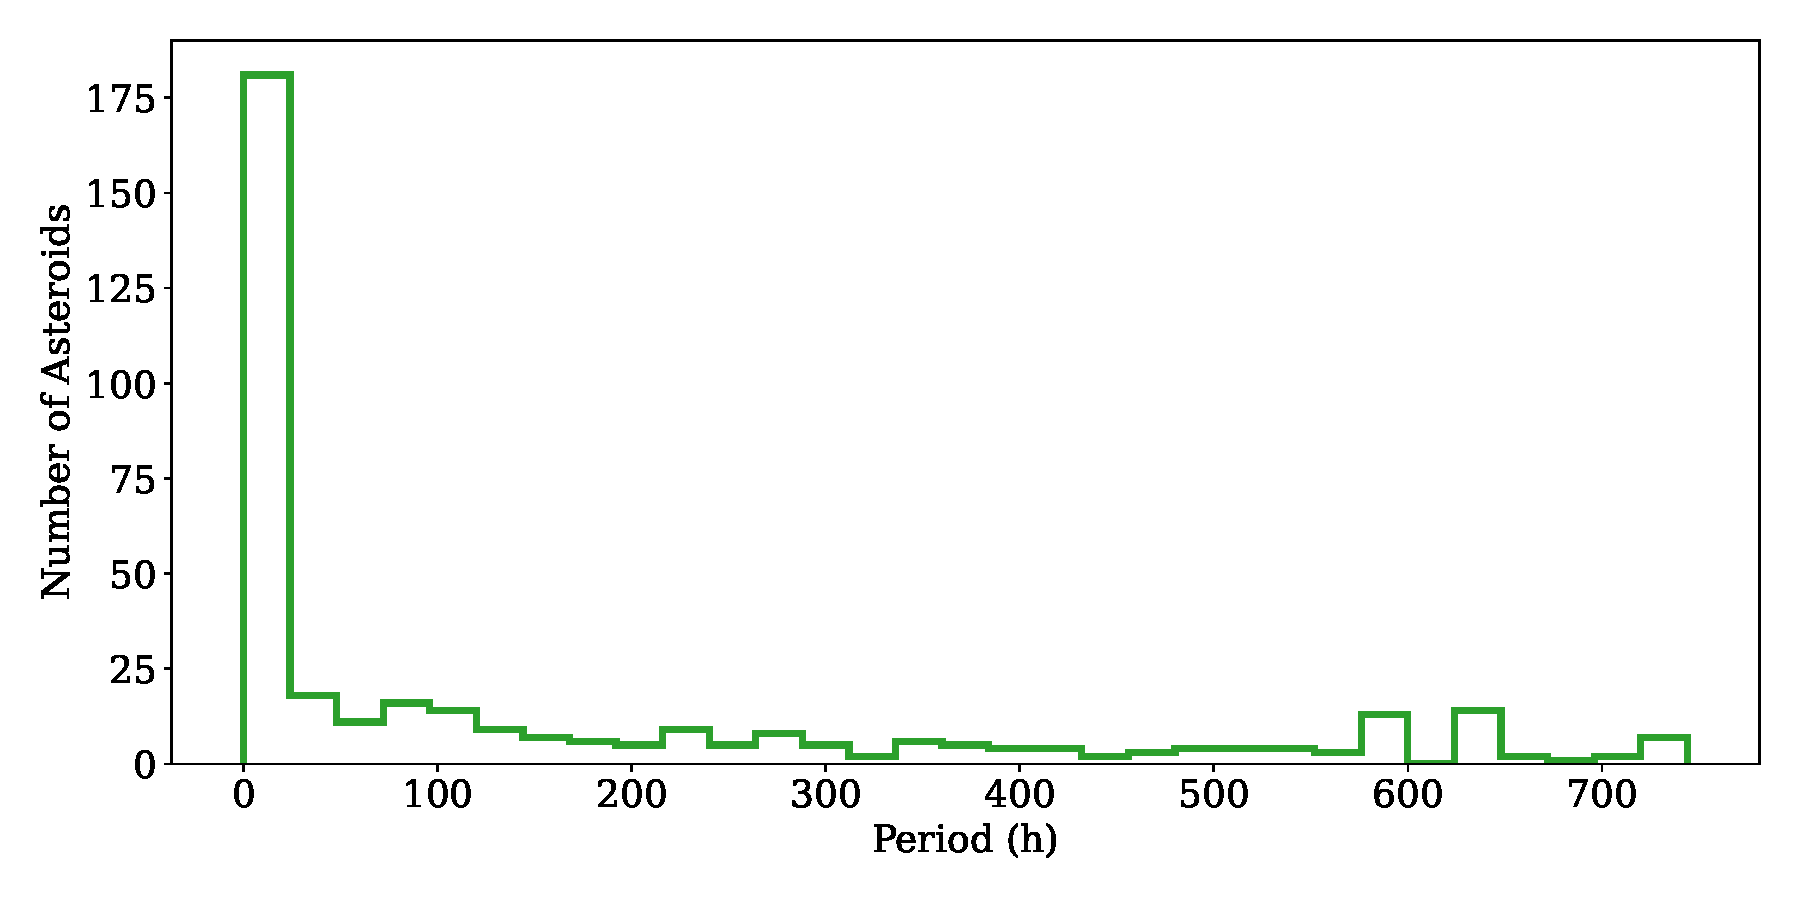
\includegraphics[width=\textwidth]{./Figures/perDistr.pdf}
  \caption[Period Distribution]{The distribution of rotation periods in \qty{24}{\hour} (\qty{1}{\day}) bins for all the asteroids that passed the quality checks.}
  \label{Fig:PerDistr}
\end{figure}

For the 374 asteroids that pass the quality checks, reliable rotation periods are obtained.
\autoref{Fig:PerDistr} shows the distribution of these rotation rates.
The period plotted is double the detected period, to account for the double-peaked nature of most lightcurves.
The mode of the distribution is a period less than \qty{1}{\day}, by a factor of 10 over periods in the \qtyrange{1}{2}{\day} bin, the \nth{2} most populated range.

\begin{figure}[!t]
  \centering
  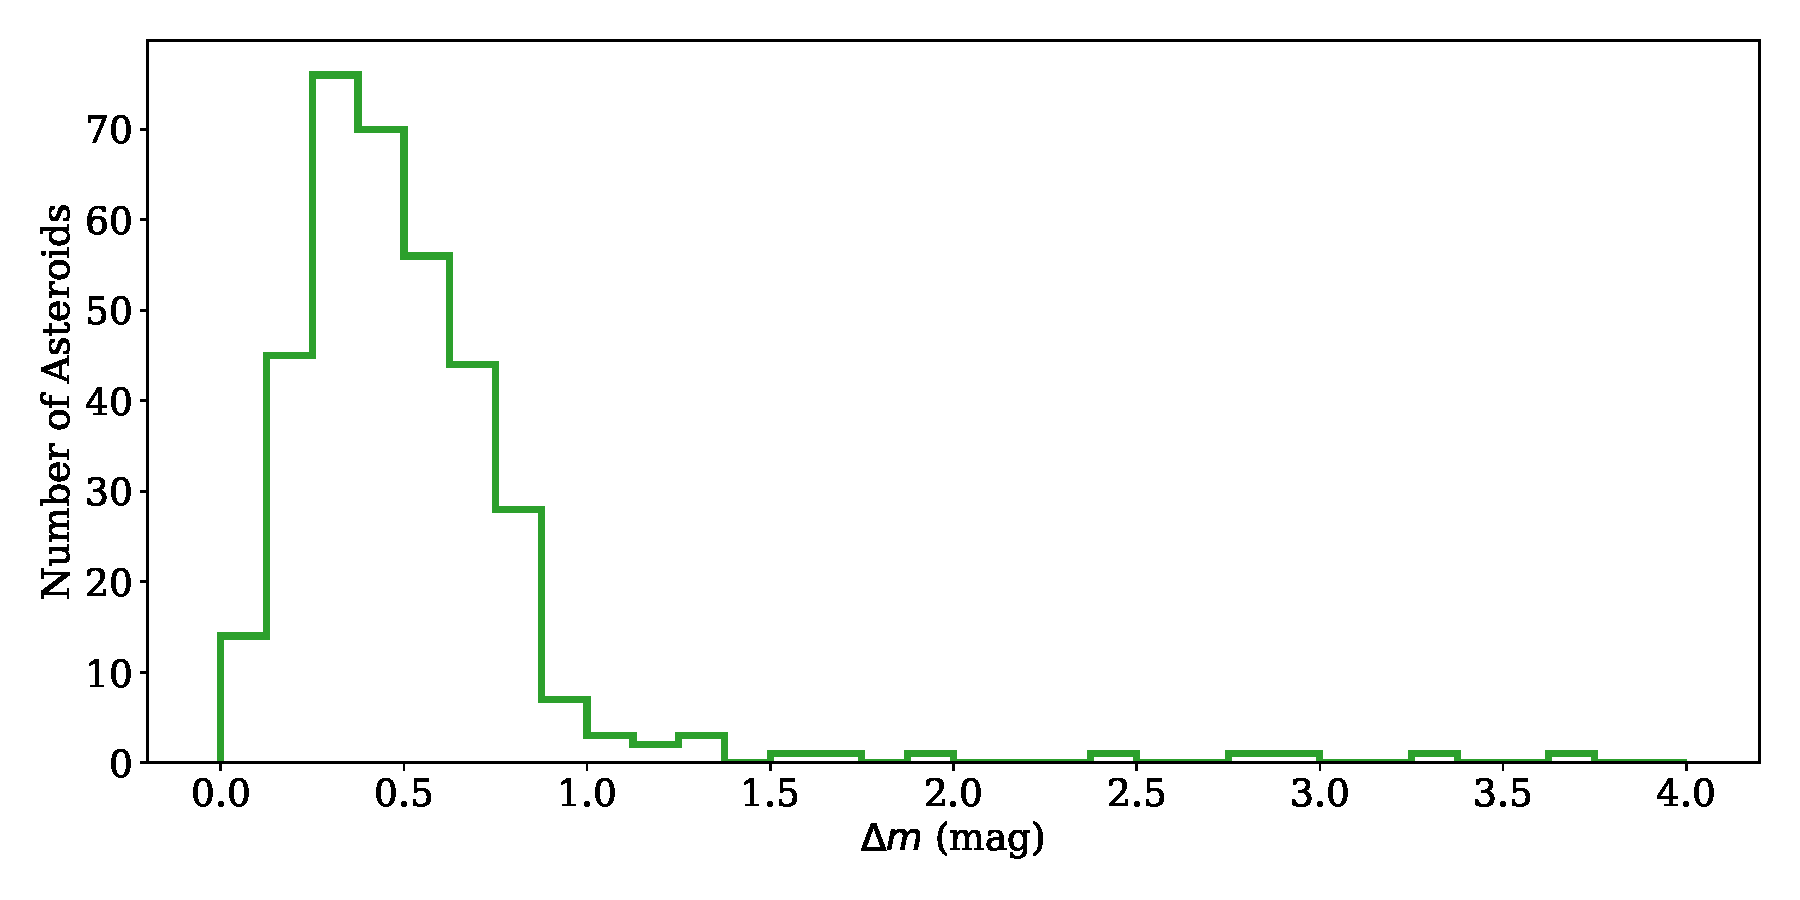
\includegraphics[width=\textwidth]{./Figures/delMagDistr.pdf}
  \caption[Amplitude Variation Distribution]{The distribution of amplitude variation for all the asteroids that passed the quality checks.
    The data are binned in steps of $\frac{1}{8}$ \unit{\mag}.
  }
  \label{Fig:ampDistr}
\end{figure}

The distribution of the amplitude of the lightcurves is given in \autoref{Fig:ampDistr}.
The peak of the distribution at $\frac13$ \unit{\mag} and is right skewed.
The high $\Delta m$ values are from lightcurves of dubious quality.
Manually checking the analysis, it is clear that these asteroids above $\Delta m =\qty{1.5}{\mag}$ have all been affected contamination in their lightcurves, and have untrustworth photometry.
Some examples are given in the appendix, Figures \ref{ApFig:Takashimizuno} \ref{ApFig:Wuyeesun} and \ref{ApFig:Locarno}

It is unclear how to avoid such contamination.
For some objects, analysis of the residuals could show a pattern that leads to a period and possible fit of a model, but this is not the case for all of them.
For only one sector worth of data, it was manageable to preform a manual check on these few outliers.
This will not be the case for all the whole dataset \texttt{TESSELLATE} will analyse.


\begin{figure}[!h]
  \centering
  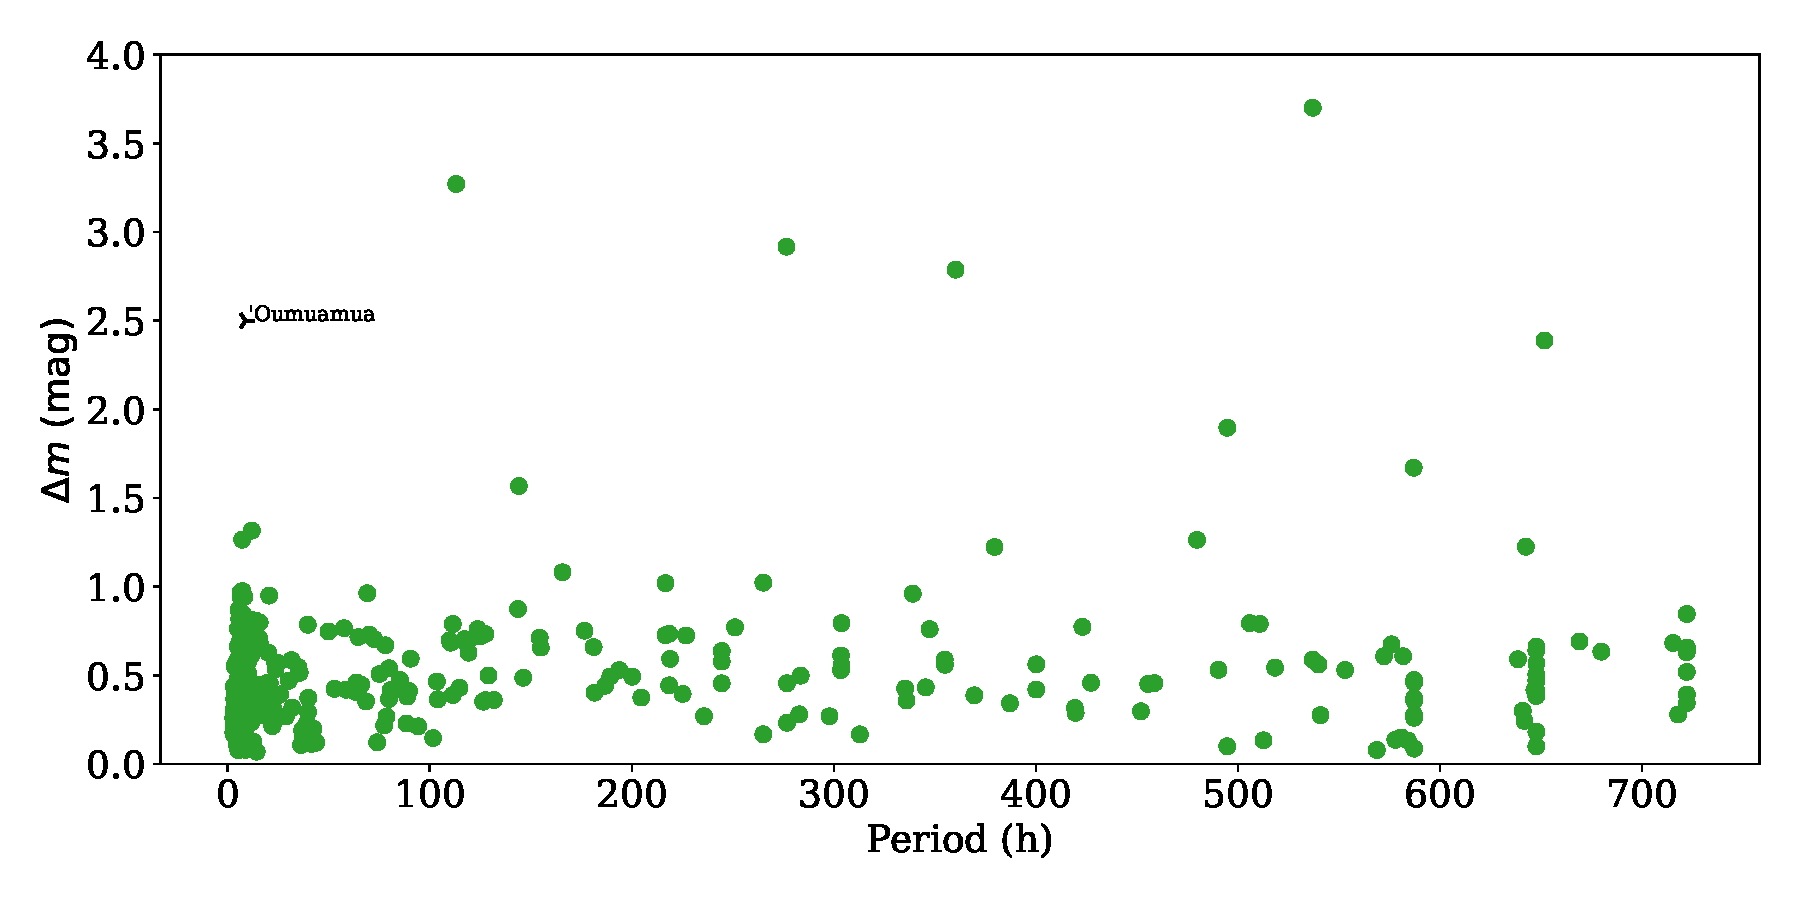
\includegraphics[width = \textwidth]{./Figures/QualPervsAmp1I.pdf}
  \caption[Amplitude of Variation against Rotation Period]{The amplitude of variation in the model from the period analysis against the calculated rotation period.
    This is for all 374 %!CHECK
    objects that pass the quality checks.
  }
  \label{Fig:perVSamp}
\end{figure}


Comparing the rotation period to the $\Delta m$ is insightful and is shown in \autoref{Fig:perVSamp}.
All 374 of the objects that pass the quality checks are plotted here, and no trend is observed.
The variation is quite constant across the range of rotation periods, although there are fewer objects at longer periods.

The modes of each of the distributions in \autoref{Fig:PerDistr} and \autoref{Fig:ampDistr} do not fully overlap, as indicated by \autoref{Fig:perVSamp}.
Those asteroids with rotation periods $<\qty{24}{\hour}$ have a wide range of amplitudes.
Conversely, the objects with a $\Delta m \approx 0.3$ span the entire period range.

The position in the space of these axes for \omuamua is shown in \autoref{Fig:perVSamp} by the black caltrop and is highlighted with text.
1I's rotation period of \qty{8.67(0.34)}{\hour} from \citet{Belton2018} and a $\Delta m$ of \qty{2.5}{\mag} from \citet{Meech2017} are used.
There are some asteroids with a larger $\Delta m$ but, as discussed, these are not trustworthy.


\section{Discussion}\label{Sec:Disc}

\subsection{Comparison to Literature Data}\label{SubSec:LitComp}

\begin{figure}
  \centering
  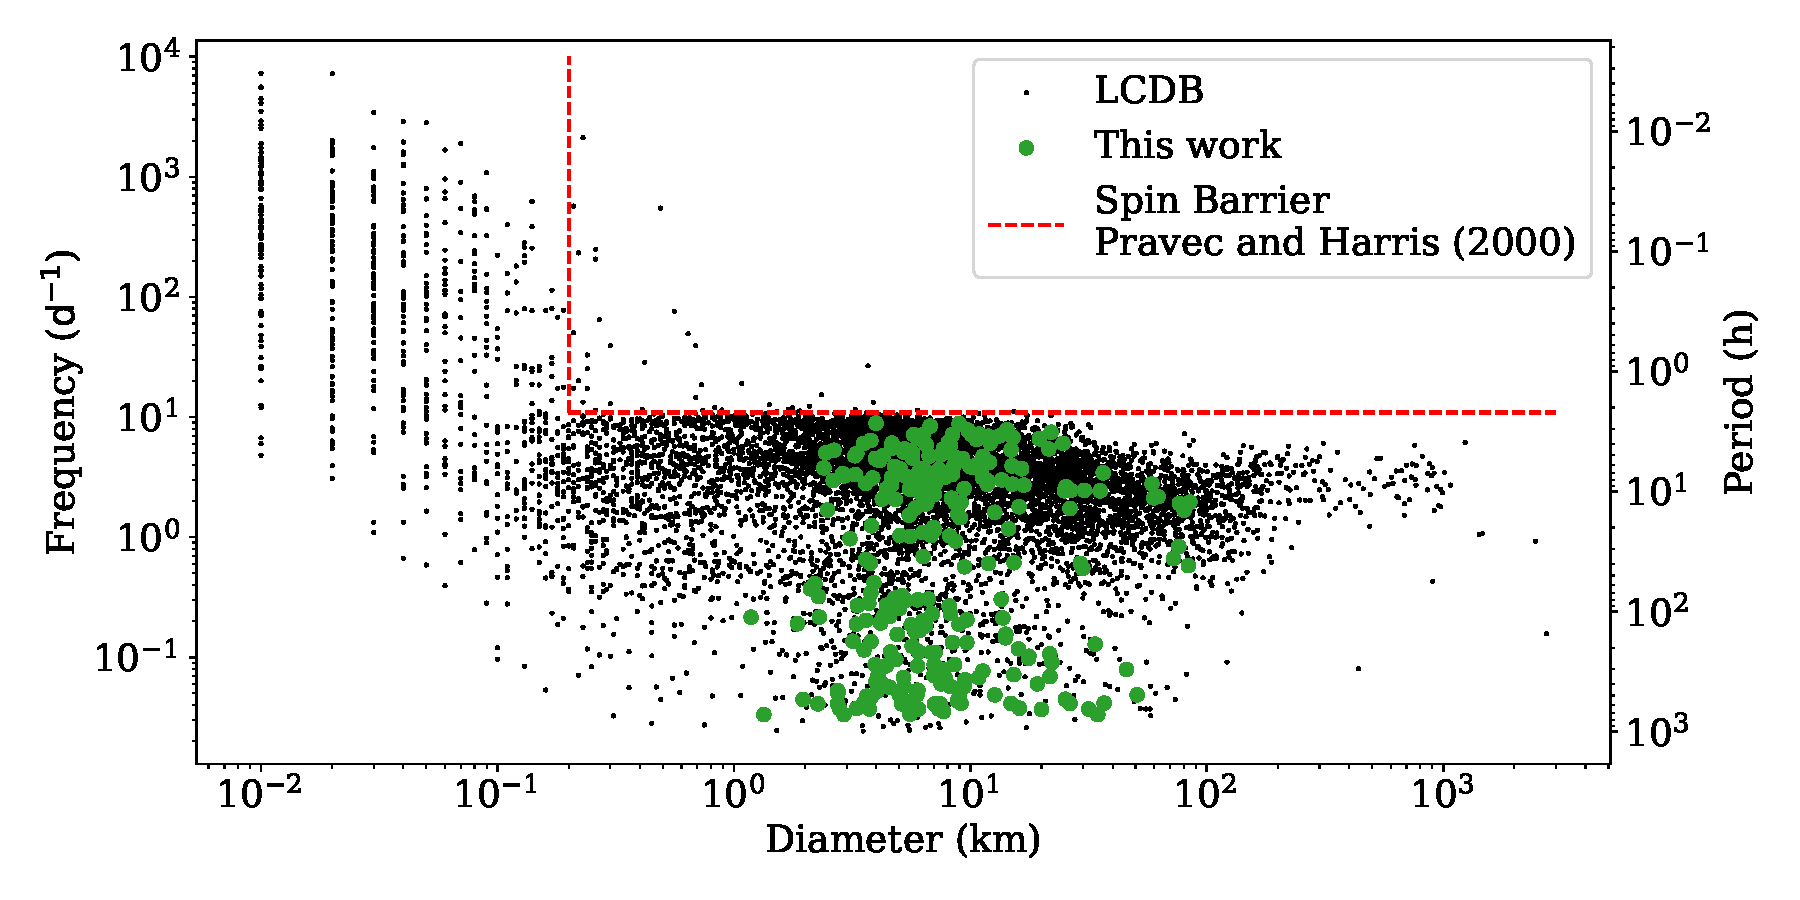
\includegraphics[width=\textwidth]{./Figures/Diam-FreqPlotThisWork.pdf}
  \caption[\autoref{Fig:FreqVsDiam} updated by this work and NEOWISE]{This work's addition to \autoref{Fig:FreqVsDiam} and the LCDB of \citet{Warner2009}. The diameters are from NEOWISE where available.}
  \label{Fig:FreqDiamUpdate}
\end{figure}

\autoref{Fig:FreqDiamUpdate} overlays the rotation periods calculated here with those presented in \autoref{Fig:FreqVsDiam}, the LCDB of \citet{Warner2009}.
269 of the asteroids that pass the quality checks have diameters available. 
The sizes are from the near-Earth object wide-field infrared survey explorer (NEOWISE) V2.0 database \citep{Masiero2011, NEOWISE2019}.
It is only this sub-sample of the 374 asteroids with derived periods that are plotted in \autoref{Fig:FreqDiamUpdate}.
The diameters in the LCBD are not calculated using NEOWISE data, so there could be discrepancies in those asteroids that have calculated periods by this analysis and are also in the LCDB.
The NEOWISE data is self-consistent and encompasses more asteroids that the diameters from just the LCDB, so it was preferred for this figure.

It is clear that TESS struggles to determine periods for asteroids with a diameter $\lesssim \qty{1}{\kilo \metre}$.
This is most likely due to these bodies being too dim for the telescope.
Those that are seen have not passed the quality checks imposed upon them.

The spin barrier of \citet{Pravec2000} is not violated by any of the periods calculated.
The quality checks to do not exclude a violation, as the spin barrier is at $\sim \qty{2.4}{\hour}$, and the checks only remove periods $<\qty{1}{\hour}$.
This cadence of FFIs have the ability to probe the forbidden region, to find more objects that violate the spin barrier.
However, none were found in sector 29.

\begin{figure}[!t]
  \centering
  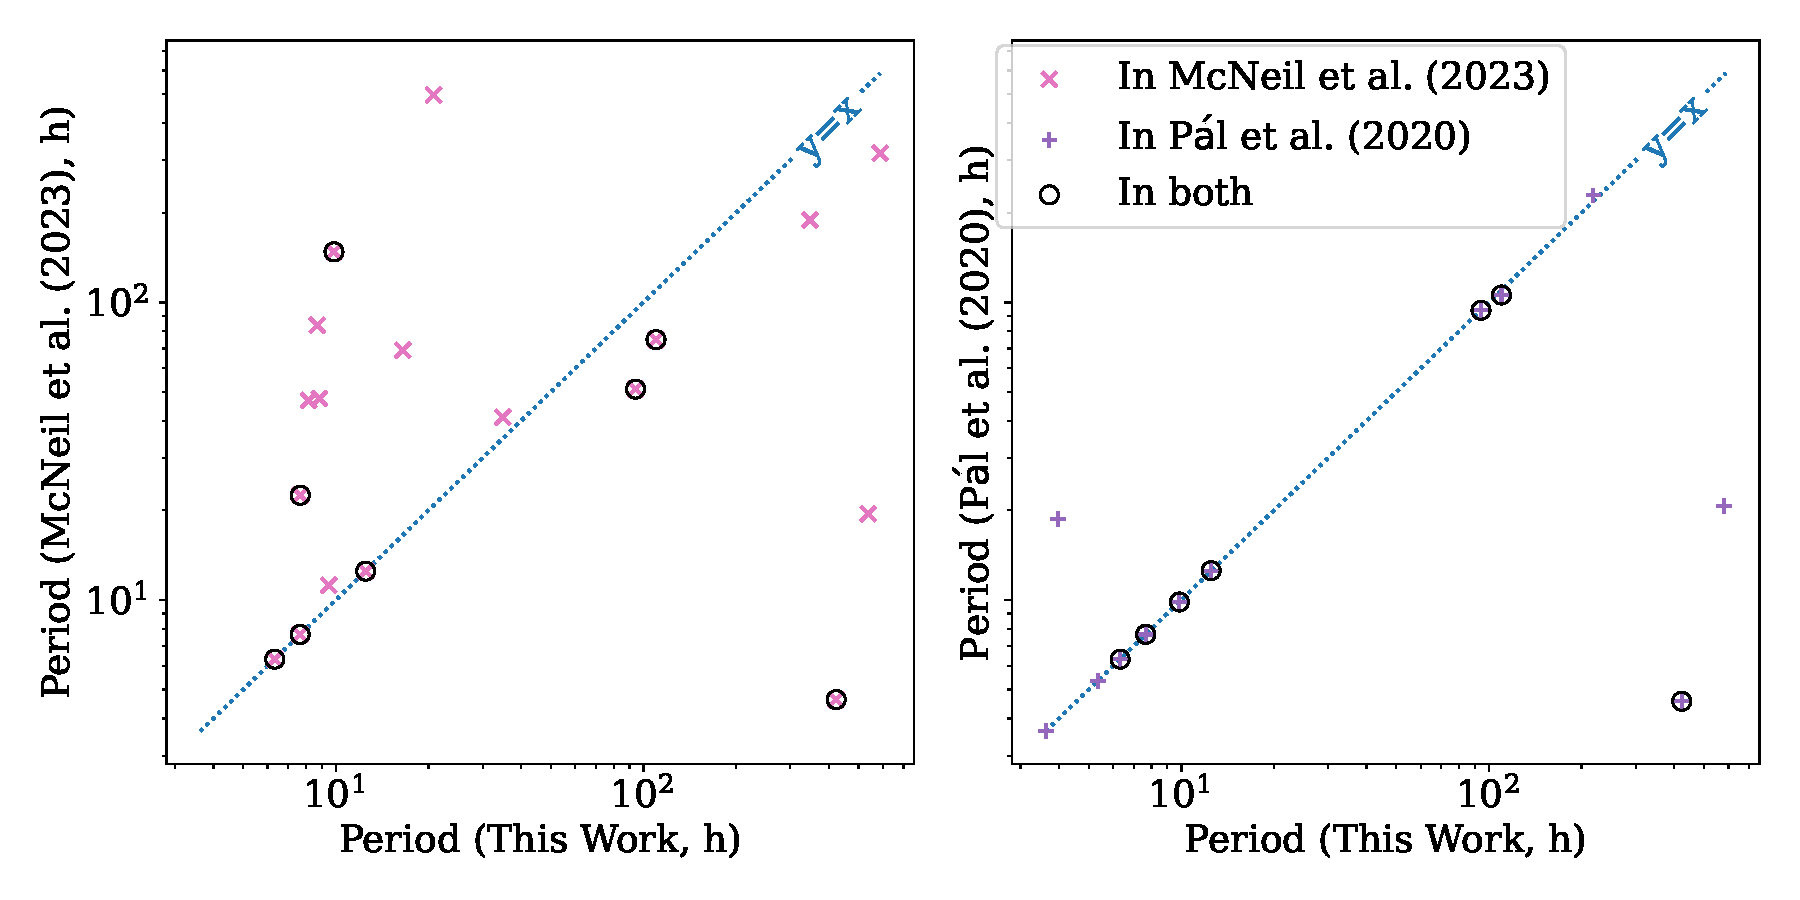
\includegraphics[width=\textwidth]{./Figures/M23andP20Comp.pdf}
  \caption[Comparison to TESS periods from the Literature]{Comparison of the rotation periods I have calculated to the publicly available data from \citet{McNeill2023} (left, pink crosses) and \citet{Pal2020} (right, purple pluses). The asteroids that are in all three are highlighted with black rings around the symbols.
    A $y=x$ line is plotted to guide the eye.}
  \label{Fig:TESSLit}
\end{figure}

As mentioned in \autoref{SubSec:TESS}, this is not the first work analysing asteroids in TESS data.
This work has 18 objects in common with \citet{McNeill2023} and 13 asteroids with the data of \citet{Pal2020}.
A comparison of the calculated periods is displayed in \autoref{Fig:TESSLit}.
There is agreement in the derived periods for some objects in both datasets, as seen by the points on or near the $y=x$ line in each sub-plot.
Both literature datasets are in broad, but not complete, agreement for the asteroids they both measure \citep[see the comparison in][]{McNeill2023}, so it is not surprising that this work is not in complete agreement with either of them.

It does not appear that my calculated periods are biases towards longer or shorter values.
Both in of these comparison datasets, and in the check against the LCDB in \autoref{Fig:LCDBcomp}, there are periods on either extreme.
Sometimes the periods found here are much shorter than those found in the external data, and others are much longer.
However, this is in about equal proportions.
The sample size is too small to make any statistical statements, once again more sectors need to be analysed for a larger overlap to be found.

There are eight objects that appear in all three datasets, and are highlighted by black circles around the data points.
Two of them lie almost directly on top of each other in the \citeauthor{Pal2020} data on the right panel of \autoref{Fig:TESSLit}, but there is a difference between them on the left-hand side, the \citeauthor{McNeill2023} data.
This intersection is shown again in \autoref{Tab:AllPers}, where it is more clear how well some of these data line up.
Both (13364) 1998 UK20 and (16151) 1999 XF230 have the same rotation period measured in all three analyses.

The period calculated for (36240) 1999 VN44 is two orders of magnitude larger than either of the two previous studies.
A spot check (\autoref{ApFig:1999VN44}) shows that the average flux of the object is low, barely passing the quality check.
This is yet another indication that these checks are not perfect.
A comparison to these datasets of \citeauthor{Pal2020} and \citeauthor{McNeill2023} was not made until after the checks were finalised, in order to limit the biases from small sample sizes. 

I seem to calculate similar periods to \citeauthor{Pal2020} more frequently than with \citeauthor{McNeill2023}, but again this is too small of a sample size.
Only one sector of data is analysed here, they both measure periods for the same 13 sectors. 
When more data has been run through both \texttt{TESSELLATE} and my pipelines, then the number of intersecting objects will increase, and a more thorough comparison can be done.

\begin{table}[!t]
  \centering
  \caption[TESS Literature Comparison Table]{The eight asteroids have rotation periods in this work rounded to two decimal places. Their periods as calculated by \citet{Pal2020} and \citet{McNeill2023} are also given. All periods are measured in hours (\unit{\hour})} \label{Tab:AllPers}
  \pgfplotstabletypeset[
    col sep=&,
    string type,
    columns/a/.style={column name=(MPC designation) Asteroid Name},
    columns/b/.style={column name=This work},
    columns/c/.style={column name=\citeauthor{McNeill2023}},
    columns/d/.style={column name=\citeauthor{Pal2020}}
  ]{tabDat.dat}
\end{table}

The distributions of periods and amplitudes also agree with these studies. 
My \autoref{Fig:PerDistr}  show similar distributions to Figures 11 and 12 in \citet{McNeill2023} and their Figure 13 peaks a little earlier than my \autoref{Fig:ampDistr}. 
\citet{Pal2020} does not give a variation amplitude distribution, but my period distribution agrees broadly with their Figure 7.
The reliability percentage of \qty{70}{\percent} derived by comparison to the LCDB (\autoref{Fig:LCDBcomp}) is almost as high as the $\sim \qty{80}{\percent}$ of \citeauthor{Pal2020} and the $\qty{85}{\percent}$ of \citeauthor{McNeill2023}.

The limiting magnitude of the recovery fraction demonstrated in \autoref{Fig:RecovPassorFail} agrees well with other tests of \texttt{TESSELLATE}.
Concurrent work by another Honours' student \citep{MontillaHons} achieves a similar recovery fraction detection efficiency of $\sim$\nth{17} \unit{\mag}.
They have been preforming injection/recovery tests across many TESS sectors, and they find that the limiting magnitude is consistent across sectors.
The cadence of the FFIs also seems to have no effect on the depth of the images.
This is promising, as it means that asteroids will be detected to a similar depth as they are here for any further sectors processed, something I could not check myself.

\subsection{Future work}
%quality checks aren't great
It is clear from the outliers in \autoref{Fig:perVSamp} and the clearly incorrect periods of known objects in \autoref{Fig:LCDBcomp} that the quality checks have room for improvement.
Some of these checks were  taken to agree with how others analyse similar data, like the maximum period from \citet{McNeill2023}.
Others were more empirically derived, such as the minimum average flux value.
There is a delicate balance between detecting as many known periods as possible and maintaining strict enough cuts to keep unreliable periods out of the data.

The periodogram noise at the low frequency end is quite strong throughout the range of rotation periods.
Currently, it is responsible for a lot of undetected rotation rates, due to the maximum period check, and this noise region having a larger power than any signal.
Modelling this excess to try and remove the noise and boost the signal from the rotation could be done to improve the maximum power of the periodogram.
There are a few asteroids with known longer rotation periods than this check allows for, but one TESS sector will not be enough to determine those accurately.

Linking lightcurves of asteroids between sectors was not considered here, as only one sector has been analysed.
An asteroid will be in multiple sectors, as TESS has surveyed that whole sky more than once.
The different FFI cadence, as well as the large temporal gap between these observations makes it non-trivial to recover the rotation periods.
One could calculate the rotation period in each sector, and then average.
This technique once again biases against long rotation periods, which combining sectors should help with, not hinder.

Lomb-Scargle periodograms can deal with large gaps in the time data, but would require the flux values to have the same normalisation.
\texttt{TESSELLATE} is self-consistent in the data reduction for a sector, but comparing fluxes between sectors may have some difficulties.
By assuming the mean flux of the asteroid should be physically constant, subtracting this off the lightcurves before the periodogram is run, as is already done, will start to mitigate this difference. 
There are also phase and viewing angle effects on the lightcurve that are important to correct for with large time gaps. %????
These were not considered for the single sector analysis because the change in these values is not significant over a month.

TESS is sensitive to many classes of solar system objects, as seen in \autoref{Fig:AEI} and \autoref{Fig:NumPerClass}. 
This class agnostic approach is beneficial for gathering rotation statistics across a wide range of objects. 
Asteroids physically further away, such as the Jupiter Trojans, will have their detections biased towards the larger, brighter objects, but this is the case of any survey.
While it is not a TESS specific problem, the high limiting magnitude found here does impose a cut-off in the detection of objects to an even larger size. 

High-cadence imaging of all classes of asteroids will be helpful, as missions are being sent to further away populations.
For example, the Lucy mission \citep{Olkin2021} is en route to the Jupiter Trojan asteroids.
None of the targets are in sector 29, but they will be in a TESS sector. 
Extra knowledge of their properties from the TESS data would enhance the analysis of the flybys.


\section{Conclusion}\label{Sec:Conc}

This work has analysed the asteroid population in sector 29 of TESS.
Asteroid positions and properties have been gathered from public sources, \texttt{SkyBoT} and \texttt{JPL Horizons}.
These positions have been interpolated to match the cadence of TESS, \qty{10}{\min} for the sector analysed here. 
This interpolation has been shown to be accurate to within a TESS pixel.
The COM of a small region around the interpolated position, aperture photometry was performed on this position, using a \texttt{TESSELLATE} standard \qty{1.5}{\px} aperture. 
These lightcurves then underwent minor cleaning to make sure there was no double counting of any position, and no stellar contamination.

A Lomb-Scargle periodogram was used to detect the periods of each object. 
From the model that \texttt{Astropy} determined was the best fit to the data, a $\Delta m$ was calculated to quantify the amplitude of the lightcurve. 
The distributions of these broadly agree with the literature. 

Of the 5664 objects with $V<\qty{20}{\mag}$ in found in sector 29, the rotation properties of 374 asteroids are calculated. 
These are the objects that have met all the requirements placed on their lightcurve and periodogram, and the checks were found to be \qty{70}{\percent} accurate.
59 of these asteroids have rotation periods documented in the LCDB already \citep{Warner2009}.
315 new asteroid rotation periods have been determined, as well as the amplitude of the variation in the lightcurve, \qty{80}{\percent} of the total asteroids that pass the checks.

Some bodies appear to have more extreme variation of their lightcurves that the unusual \omuamuans.
These were checked and have contamination in the lightcurves. 
This contamination has managed to pass undetected through sigma-clipping and other quality checks on the periodogram. 
There is evidently a slight issue with my checks 


I have shown that \texttt{TESSELLATE} detects asteroids far less often than they appear in the FFIs.
Most objects are matches $<100$ times, while the forced photometry lightcurves average more than 2000 observations. 
Those that are matched to TESSELLATE detections can be filtered out of further transient searches. 
The forced photometry detects more than \qty{50}{\percent} of asteroids brighter than 


The main extension of this work is to analyse more TESS sectors. 
Gathering a larger sample size is always beneficial. 
Access to more data will also help improve the quality checks on the lightcurve. 
It does take a long time to run an analysis, both the reductions and detections from \texttt{TESSELLATE} as well as the asteroid specific side of the pipeline I have developed.   
My methods are easily transferable to more sectors and upon completion of this analysis, more sectors can be analysed. 

\newpage %* Page number above here must be <=25

\section*{Acknowledgements}
\addcontentsline{toc}{section}{Acknowledgements}

I would like to thank my supervisors for the time and effort they spent making sure things were getting done, for help when I was stuck, and forever striving to improve the quality of my work. 
I would also like to thank the rest of the ASTR480 cohort for their support throughout the year. 

There are a few entities used in this work that request acknowledgement and/or citation for use of their services:

%OzSTAR wants
This work was performed on the OzSTAR national facility at Swinburne University of Technology.
The OzSTAR program receives funding in part from the Astronomy National Collaborative Research Infrastructure Strategy (NCRIS) allocation provided by the Australian Government, and from the Victorian Higher Education State Investment Fund (VHESIF) provided by the Victorian Government.

%MPC wants
This research has made use of data and/or services provided by the International Astronomical Union's Minor Planet Center.

%Horizon wants
This work has used data and/or services provided by NASA's Solar System Dynamics website, \url{https://ssd.jpl.nasa.gov/}. Specifically \texttt{JPL Horizons}: \url{https://ssd.jpl.nasa.gov/horizons/}.

%No where else worked
The figures seen in this work have been plotted by \texttt{Matplotlib} \citep{Hunter2007}, specifically Version 3.9.2 \citep{PLT3.9.2}

%Photutils wants this extra
This research made use of Photutils, an Astropy package for detection and photometry of astronomical sources \citep{Bradley2024}.

\section*{Appendix}
\addcontentsline{toc}{section}{Appendix}
\renewcommand{\thefigure}{A.\arabic{figure}}
\setcounter{figure}{0}

Here I present some more periodogram examples, Figures \ref{ApFig:Ceres} \ref{ApFig:Takashimizuno}, \ref{ApFig:Wuyeesun} and \ref{ApFig:Locarno}.
This provides context to what I claim in text especially about the contamination of the lightcurves.
As they are all so similar to \autoref{Fig:PeriodEx} and quite large, so I do not place them where they are referred to.

\begin{figure}
  \centering
  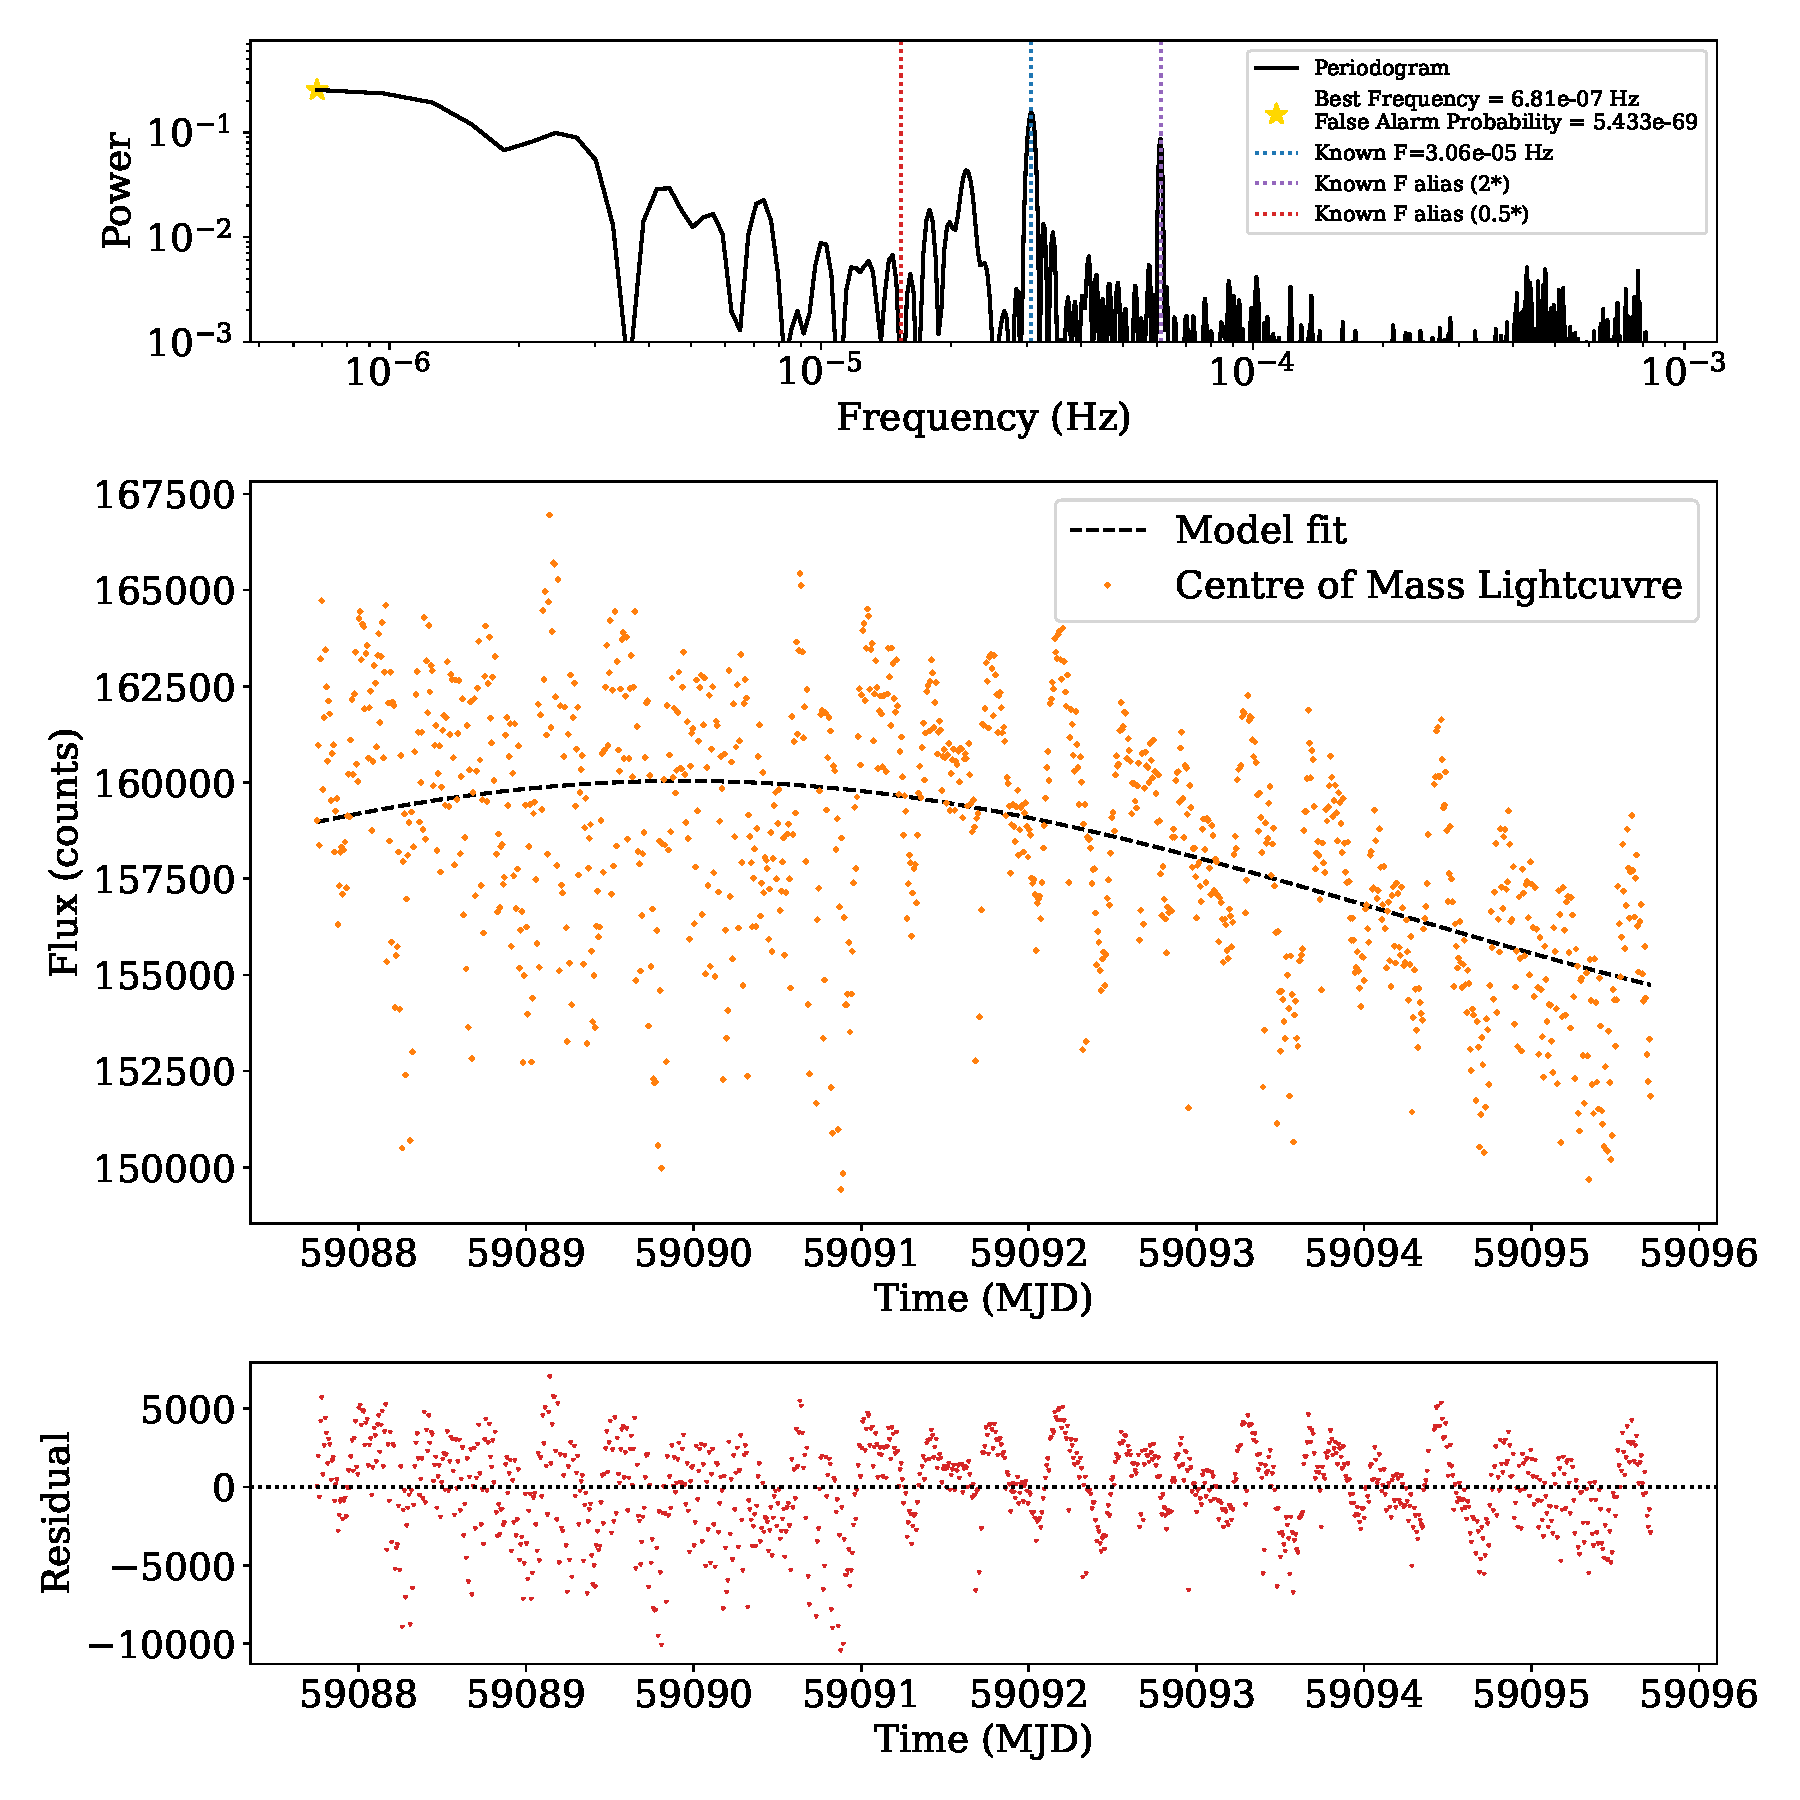
\includegraphics[width = \textwidth]{Figures/PeriodogramCeresResid.pdf}
  \caption[(1) Ceres Periodogram]{Same as \autoref{Fig:PeriodEx}, but for (1) Ceres.}
  \label{ApFig:Ceres}
\end{figure}

\begin{figure}
  \centering
  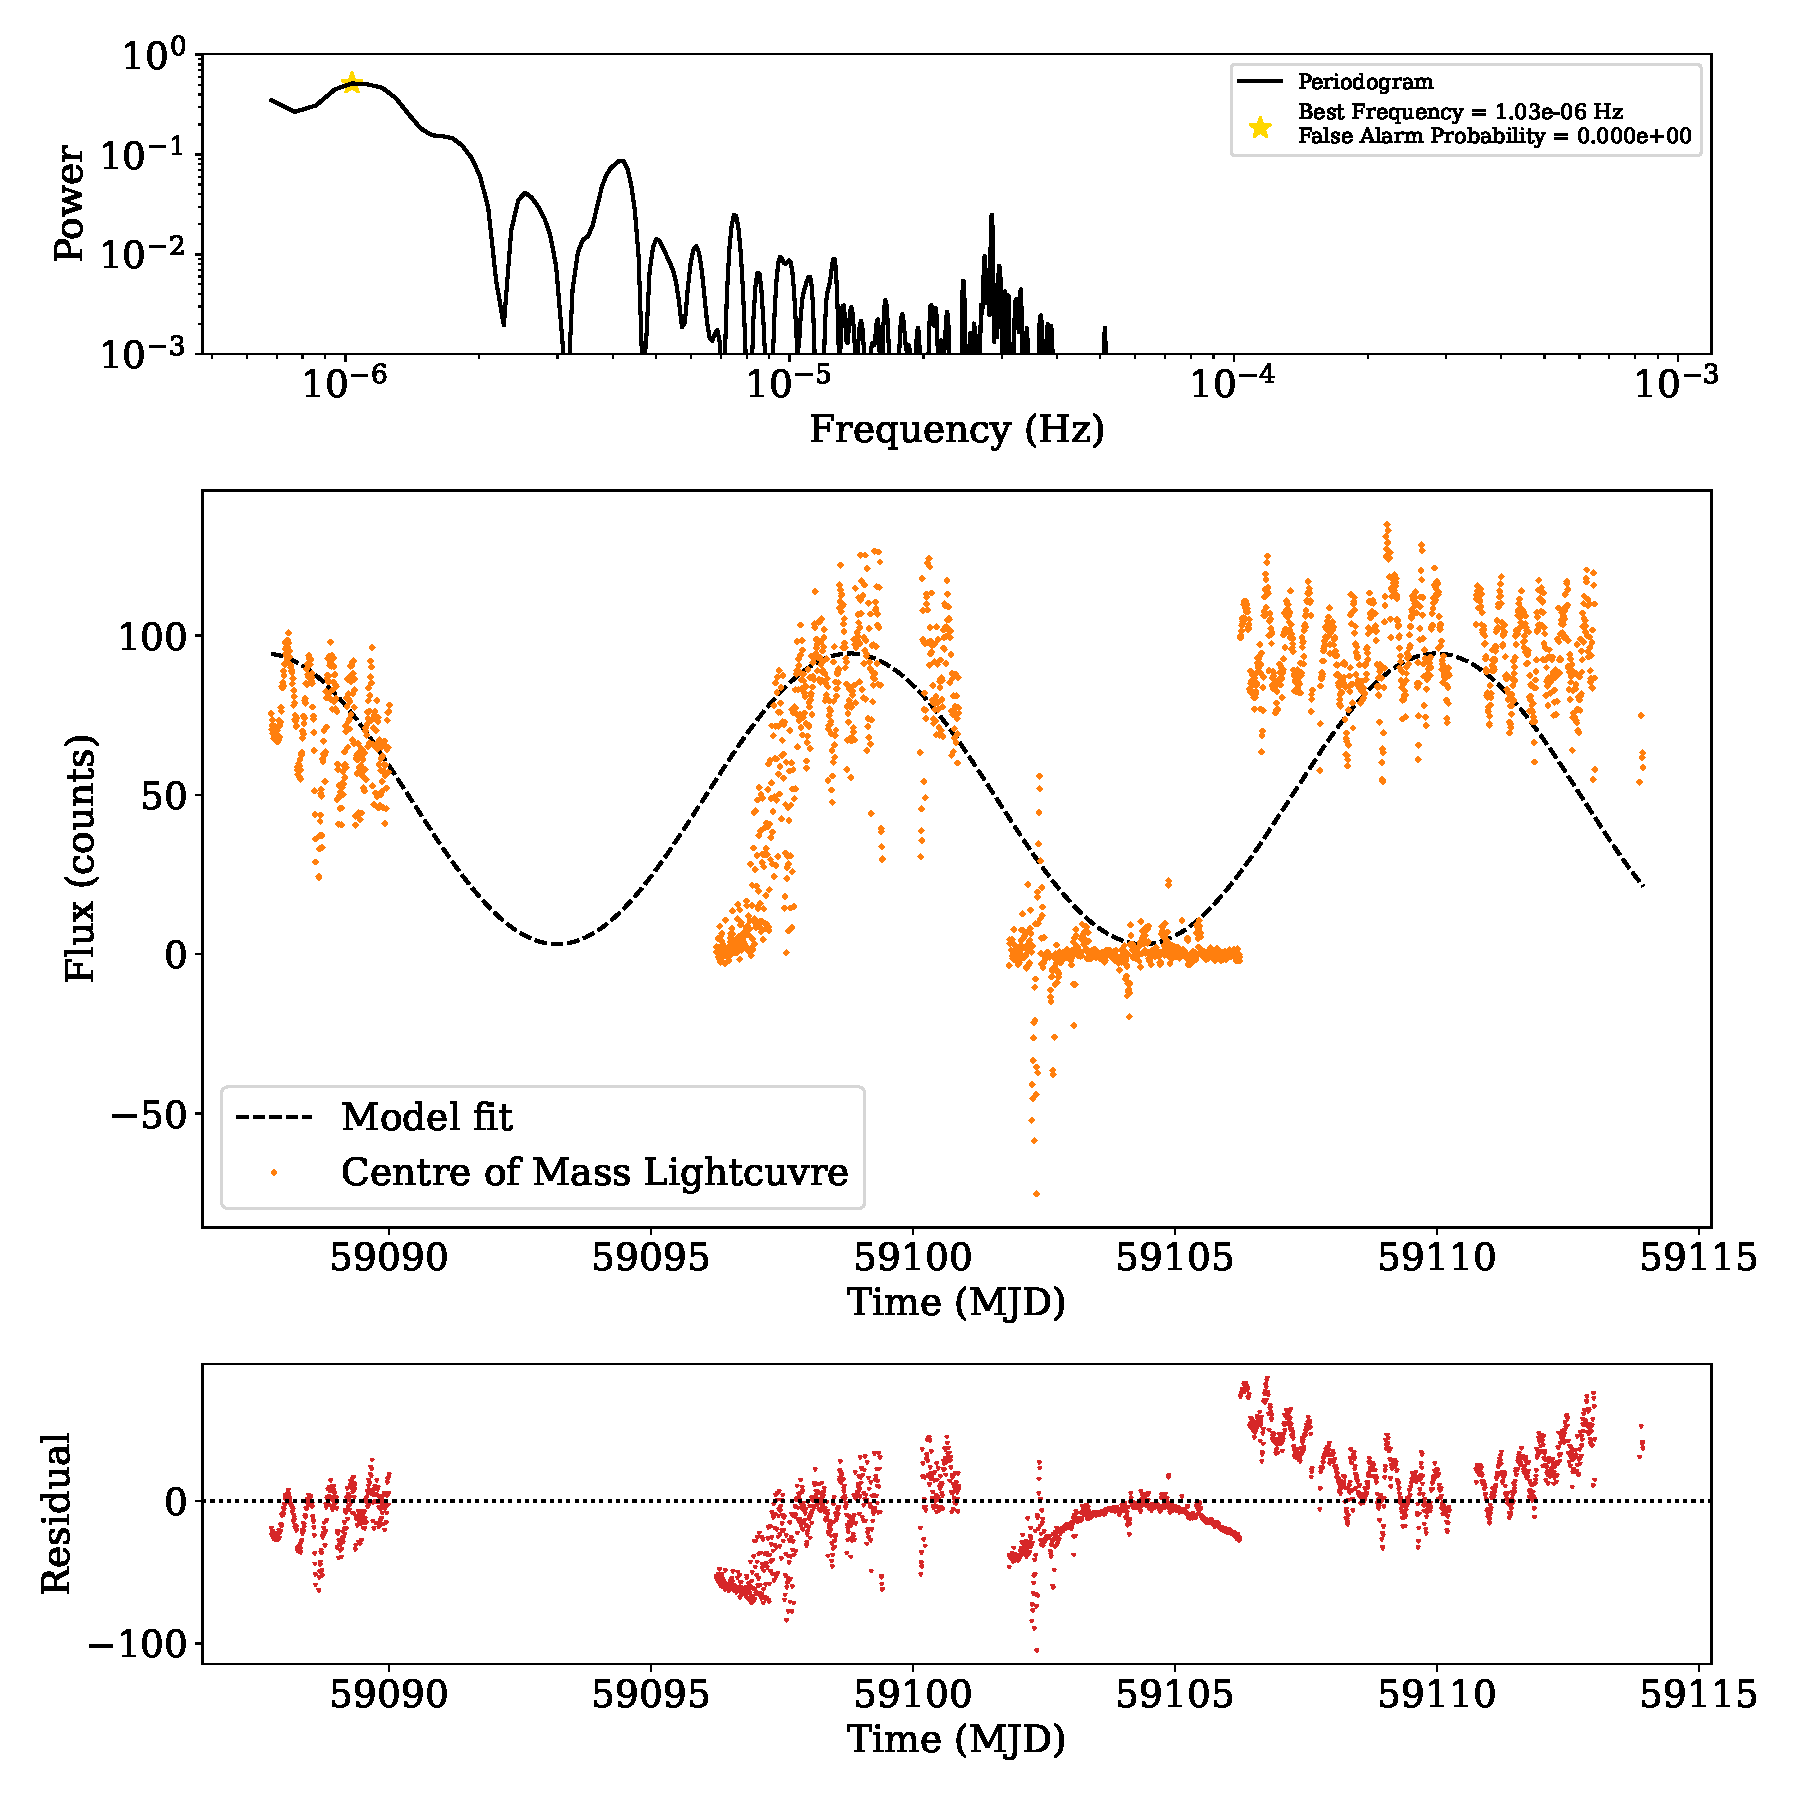
\includegraphics[width = \textwidth]{Figures/PeriodogramTakashimizunoResid.pdf}
  \caption[(6392) Takashimizuno Periodogram]{Same as \autoref{Fig:PeriodEx}, but for (6392) Takashimizuno.
  This is the highest detected variation amplitude, at $\Delta m = 3.7$.
  (6392) Takashimizuno is not in the LCDB, so a known period is not plotted.
  }
  \label{ApFig:Takashimizuno}
\end{figure}


\begin{figure}
  \centering
  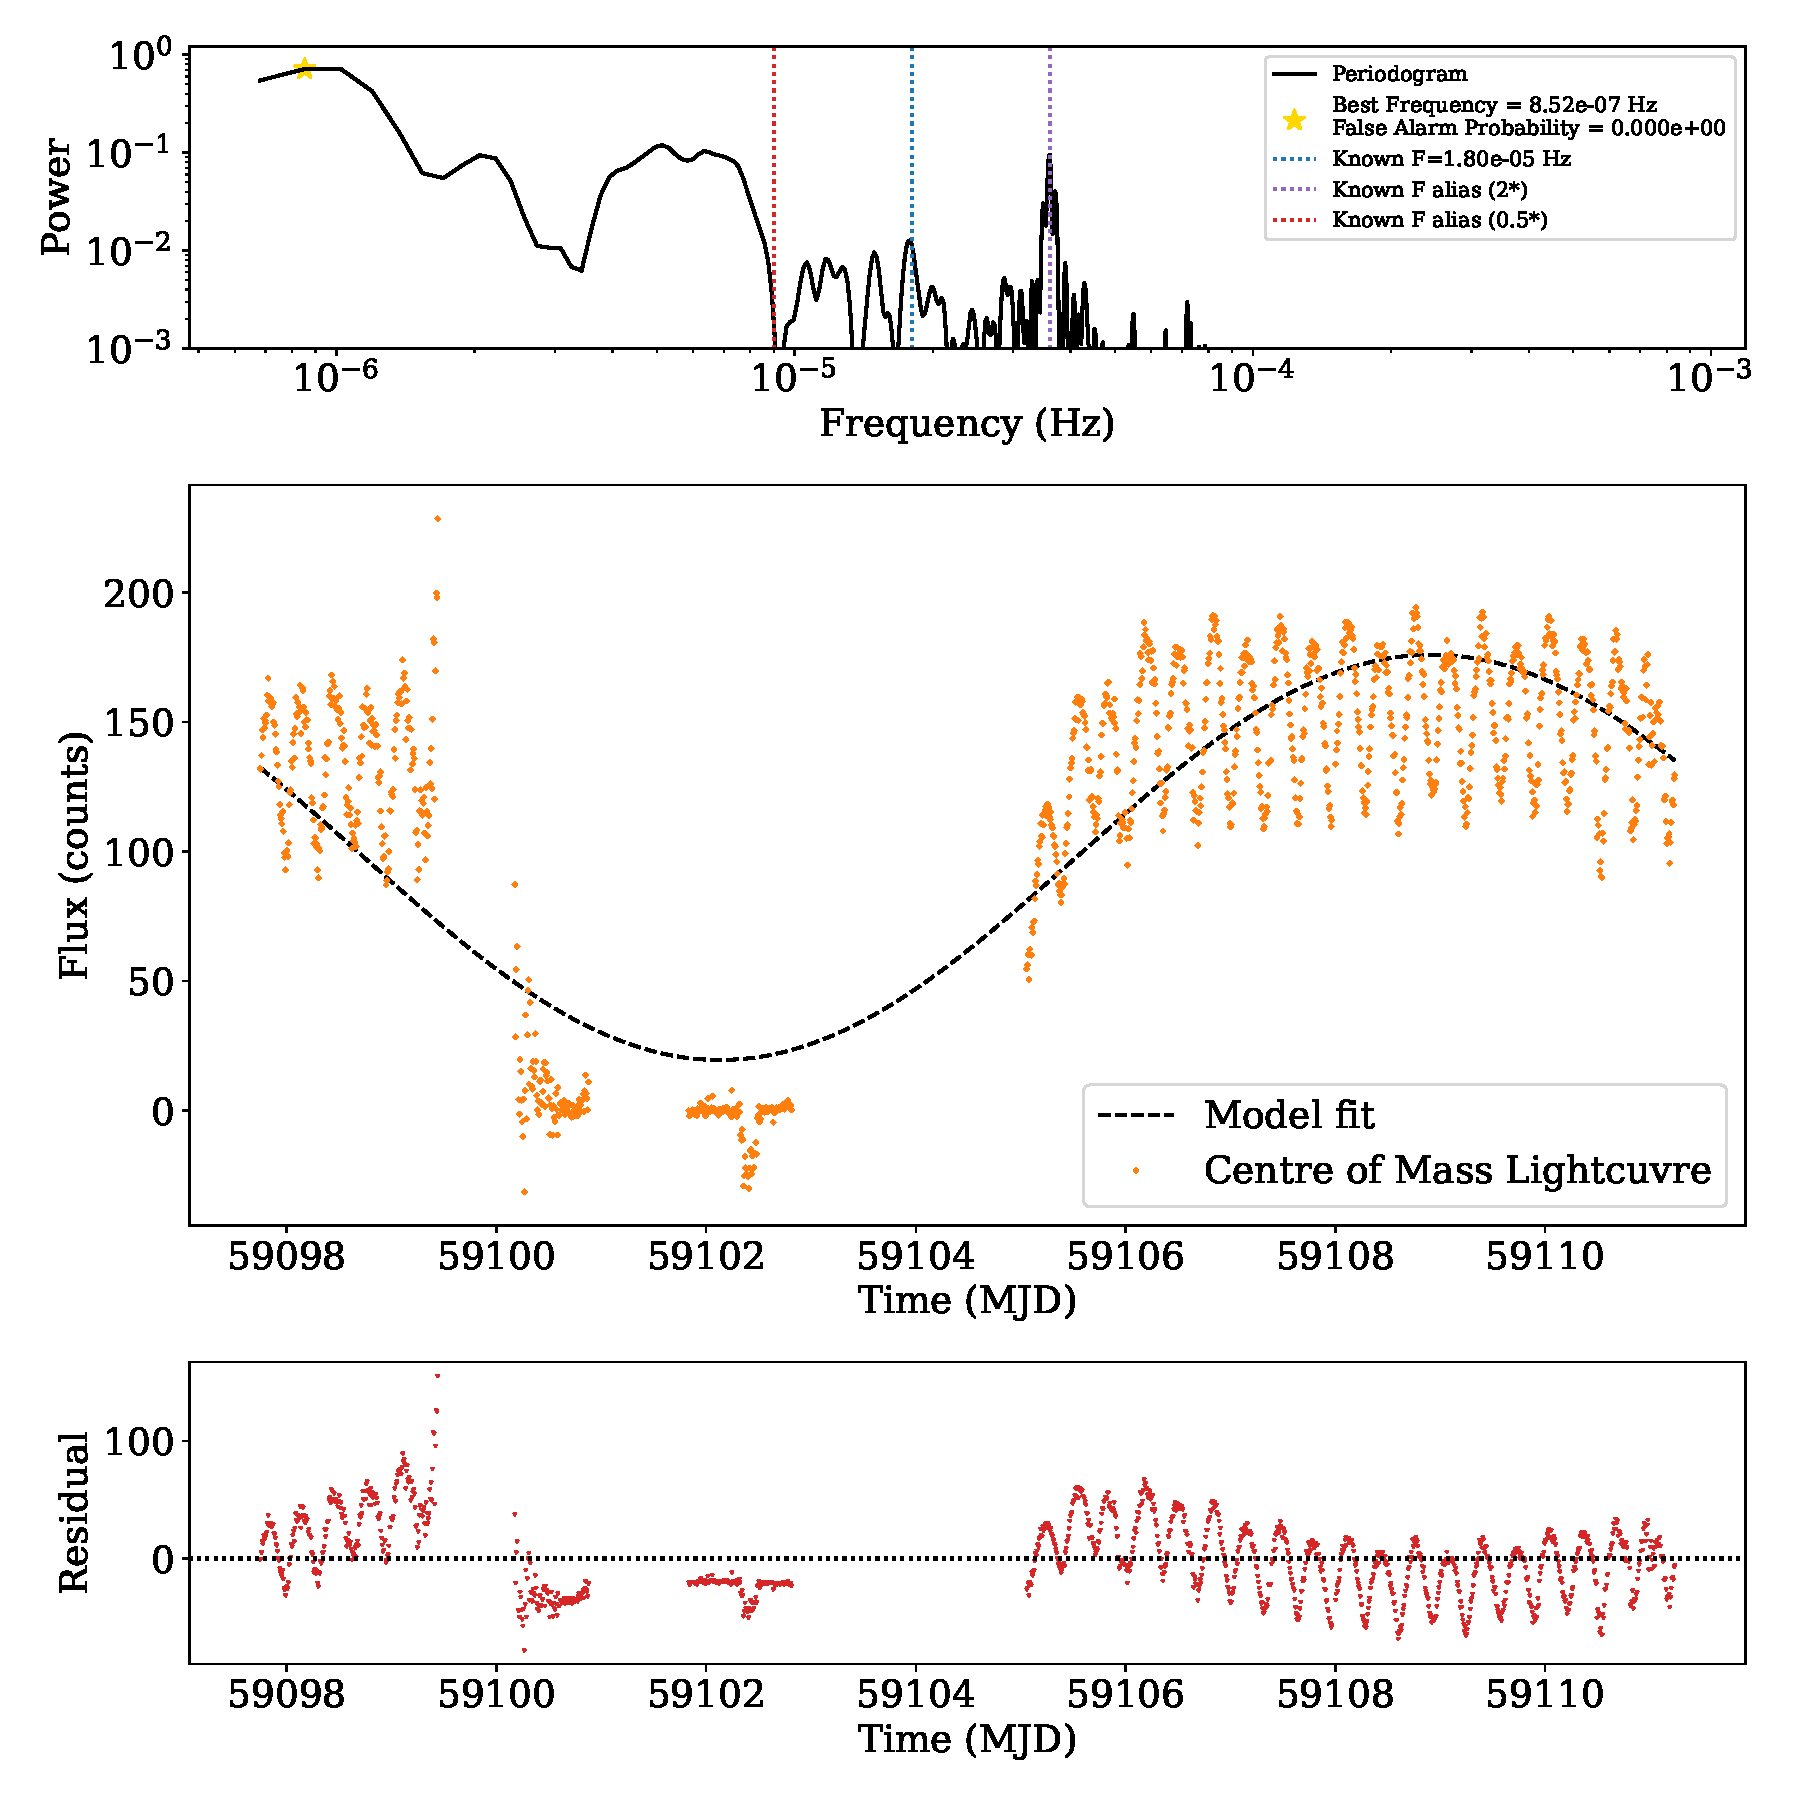
\includegraphics[width = \textwidth]{Figures/PeriodogramWuyeesunResid.pdf}
  \caption[(3570) Wuyeesun Periodogram]{Same as \autoref{Fig:PeriodEx}, but for (3570) Wuyeesun.
  This is another high variation object, and it is clear a residuals' analysis would be beneficial here, but is not attempted.}
  \label{ApFig:Wuyeesun}
\end{figure}


\begin{figure}
  \centering
  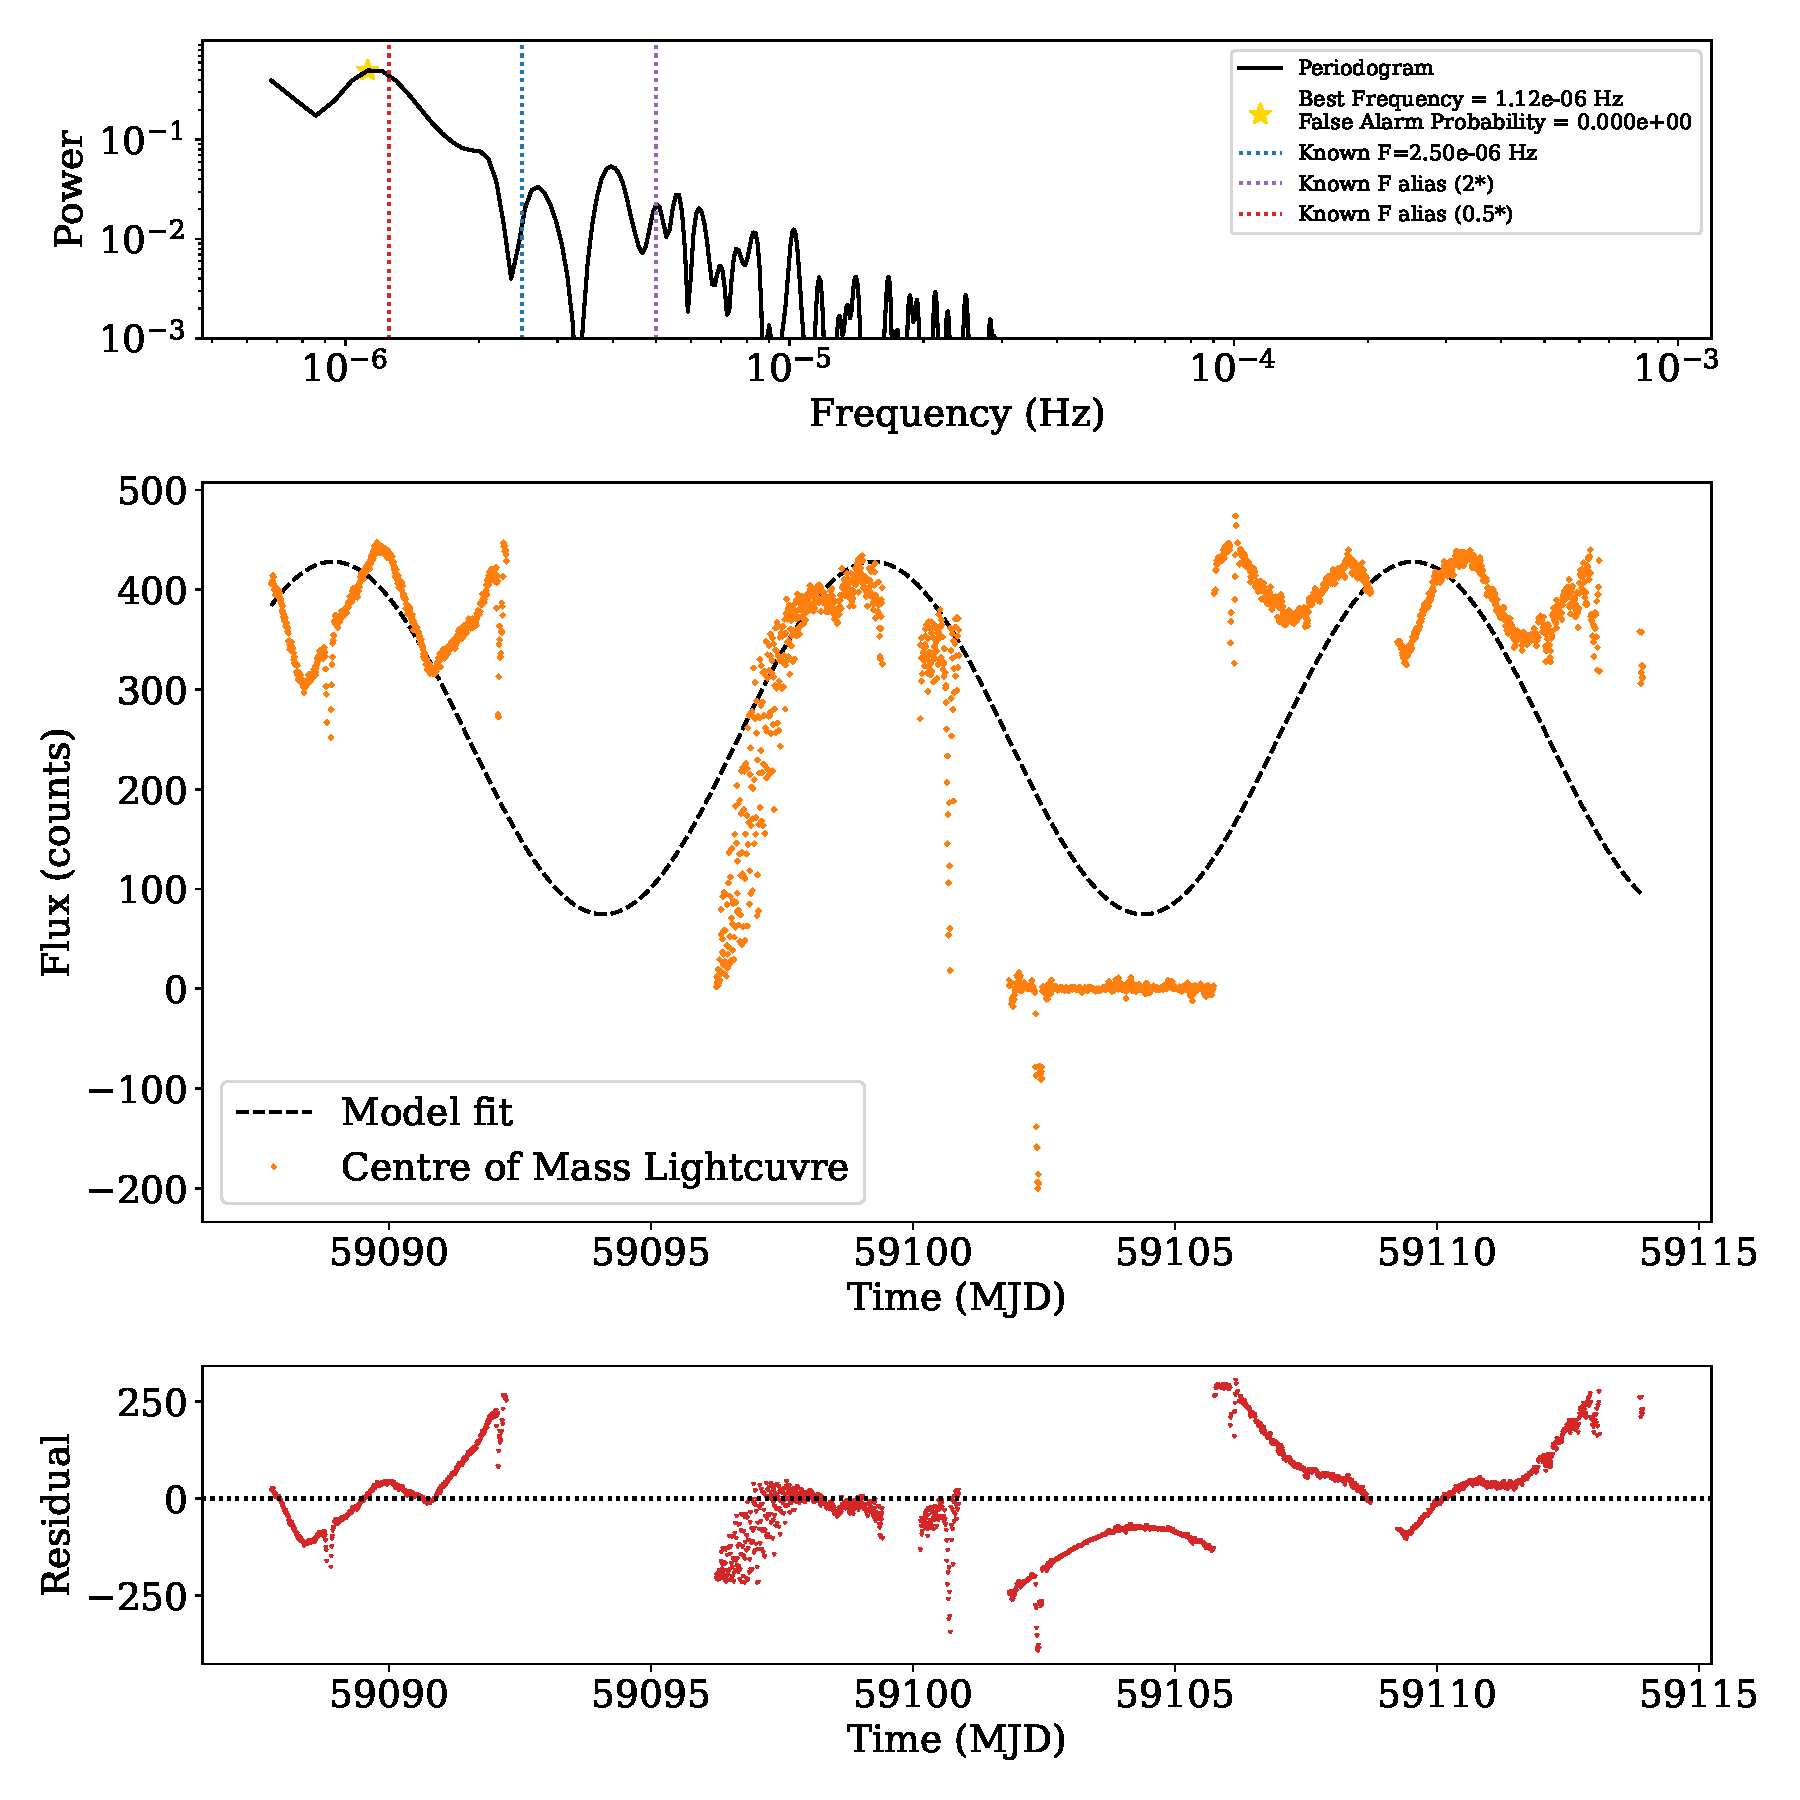
\includegraphics[width = \textwidth]{Figures/PeriodogramLocarnoResid.pdf}
  \caption[(1937) Locarno Periodogram]{Same as \autoref{Fig:PeriodEx}, but for (1937) Locarno.
  This is another high variation object, but a residuals' analysis would not help as much.}
  \label{ApFig:Locarno}
\end{figure}

\begin{figure}
  \centering
  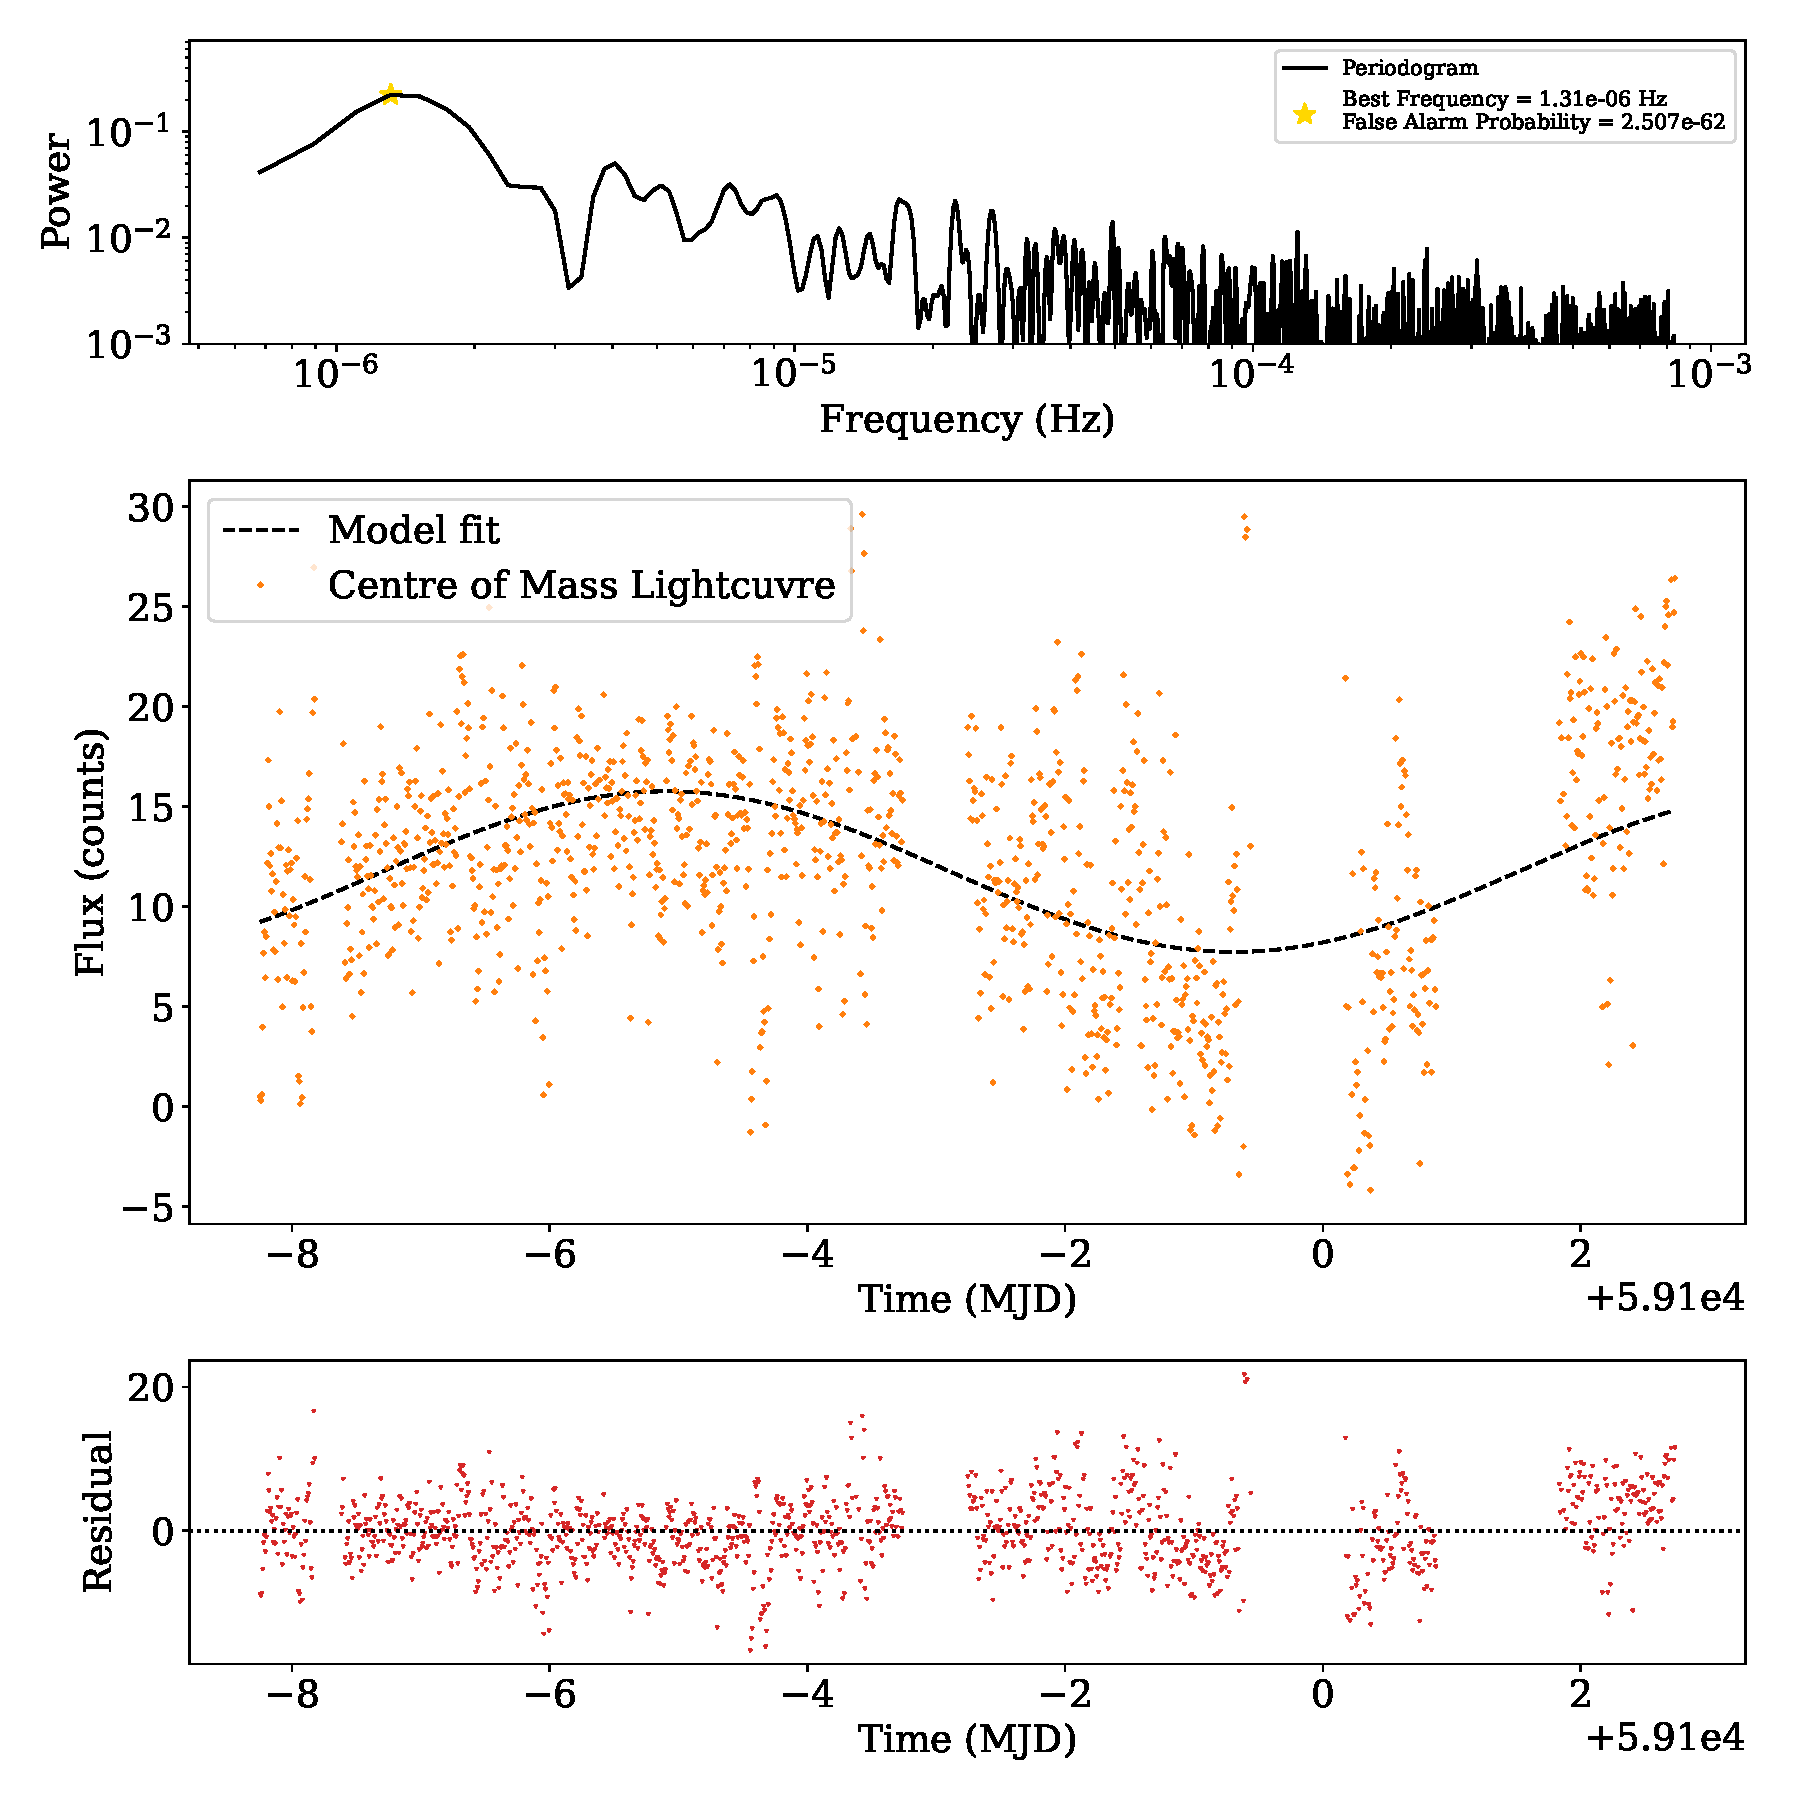
\includegraphics[width = \textwidth]{Figures/Periodogram1999 VN44Resid.pdf}
  \caption[(36240) 1999 VN44 Periodogram]{Same as \autoref{Fig:PeriodEx}, but for (36240) 1999 VN44.
  This object was in the data of both \citet{Pal2020} and \citet{McNeill2023}, but the calculated period here was not the same.}
  \label{ApFig:1999VN44}
\end{figure}

\newpage
%*Bib
\addcontentsline{toc}{section}{References}
% \bibliographystyle{jphysicsB}
\bibliography{bibfile.bib}
\end{document}



